% Options for packages loaded elsewhere
\PassOptionsToPackage{unicode}{hyperref}
\PassOptionsToPackage{hyphens}{url}
%
\documentclass[
]{article}
\usepackage{amsmath,amssymb}
\usepackage{iftex}
\ifPDFTeX
  \usepackage[T1]{fontenc}
  \usepackage[utf8]{inputenc}
  \usepackage{textcomp} % provide euro and other symbols
\else % if luatex or xetex
  \usepackage{unicode-math} % this also loads fontspec
  \defaultfontfeatures{Scale=MatchLowercase}
  \defaultfontfeatures[\rmfamily]{Ligatures=TeX,Scale=1}
\fi
\usepackage{lmodern}
\ifPDFTeX\else
  % xetex/luatex font selection
\fi
% Use upquote if available, for straight quotes in verbatim environments
\IfFileExists{upquote.sty}{\usepackage{upquote}}{}
\IfFileExists{microtype.sty}{% use microtype if available
  \usepackage[]{microtype}
  \UseMicrotypeSet[protrusion]{basicmath} % disable protrusion for tt fonts
}{}
\makeatletter
\@ifundefined{KOMAClassName}{% if non-KOMA class
  \IfFileExists{parskip.sty}{%
    \usepackage{parskip}
  }{% else
    \setlength{\parindent}{0pt}
    \setlength{\parskip}{6pt plus 2pt minus 1pt}}
}{% if KOMA class
  \KOMAoptions{parskip=half}}
\makeatother
\usepackage{xcolor}
\usepackage[margin=1in]{geometry}
\usepackage{color}
\usepackage{fancyvrb}
\newcommand{\VerbBar}{|}
\newcommand{\VERB}{\Verb[commandchars=\\\{\}]}
\DefineVerbatimEnvironment{Highlighting}{Verbatim}{commandchars=\\\{\}}
% Add ',fontsize=\small' for more characters per line
\usepackage{framed}
\definecolor{shadecolor}{RGB}{248,248,248}
\newenvironment{Shaded}{\begin{snugshade}}{\end{snugshade}}
\newcommand{\AlertTok}[1]{\textcolor[rgb]{0.94,0.16,0.16}{#1}}
\newcommand{\AnnotationTok}[1]{\textcolor[rgb]{0.56,0.35,0.01}{\textbf{\textit{#1}}}}
\newcommand{\AttributeTok}[1]{\textcolor[rgb]{0.13,0.29,0.53}{#1}}
\newcommand{\BaseNTok}[1]{\textcolor[rgb]{0.00,0.00,0.81}{#1}}
\newcommand{\BuiltInTok}[1]{#1}
\newcommand{\CharTok}[1]{\textcolor[rgb]{0.31,0.60,0.02}{#1}}
\newcommand{\CommentTok}[1]{\textcolor[rgb]{0.56,0.35,0.01}{\textit{#1}}}
\newcommand{\CommentVarTok}[1]{\textcolor[rgb]{0.56,0.35,0.01}{\textbf{\textit{#1}}}}
\newcommand{\ConstantTok}[1]{\textcolor[rgb]{0.56,0.35,0.01}{#1}}
\newcommand{\ControlFlowTok}[1]{\textcolor[rgb]{0.13,0.29,0.53}{\textbf{#1}}}
\newcommand{\DataTypeTok}[1]{\textcolor[rgb]{0.13,0.29,0.53}{#1}}
\newcommand{\DecValTok}[1]{\textcolor[rgb]{0.00,0.00,0.81}{#1}}
\newcommand{\DocumentationTok}[1]{\textcolor[rgb]{0.56,0.35,0.01}{\textbf{\textit{#1}}}}
\newcommand{\ErrorTok}[1]{\textcolor[rgb]{0.64,0.00,0.00}{\textbf{#1}}}
\newcommand{\ExtensionTok}[1]{#1}
\newcommand{\FloatTok}[1]{\textcolor[rgb]{0.00,0.00,0.81}{#1}}
\newcommand{\FunctionTok}[1]{\textcolor[rgb]{0.13,0.29,0.53}{\textbf{#1}}}
\newcommand{\ImportTok}[1]{#1}
\newcommand{\InformationTok}[1]{\textcolor[rgb]{0.56,0.35,0.01}{\textbf{\textit{#1}}}}
\newcommand{\KeywordTok}[1]{\textcolor[rgb]{0.13,0.29,0.53}{\textbf{#1}}}
\newcommand{\NormalTok}[1]{#1}
\newcommand{\OperatorTok}[1]{\textcolor[rgb]{0.81,0.36,0.00}{\textbf{#1}}}
\newcommand{\OtherTok}[1]{\textcolor[rgb]{0.56,0.35,0.01}{#1}}
\newcommand{\PreprocessorTok}[1]{\textcolor[rgb]{0.56,0.35,0.01}{\textit{#1}}}
\newcommand{\RegionMarkerTok}[1]{#1}
\newcommand{\SpecialCharTok}[1]{\textcolor[rgb]{0.81,0.36,0.00}{\textbf{#1}}}
\newcommand{\SpecialStringTok}[1]{\textcolor[rgb]{0.31,0.60,0.02}{#1}}
\newcommand{\StringTok}[1]{\textcolor[rgb]{0.31,0.60,0.02}{#1}}
\newcommand{\VariableTok}[1]{\textcolor[rgb]{0.00,0.00,0.00}{#1}}
\newcommand{\VerbatimStringTok}[1]{\textcolor[rgb]{0.31,0.60,0.02}{#1}}
\newcommand{\WarningTok}[1]{\textcolor[rgb]{0.56,0.35,0.01}{\textbf{\textit{#1}}}}
\usepackage{graphicx}
\makeatletter
\def\maxwidth{\ifdim\Gin@nat@width>\linewidth\linewidth\else\Gin@nat@width\fi}
\def\maxheight{\ifdim\Gin@nat@height>\textheight\textheight\else\Gin@nat@height\fi}
\makeatother
% Scale images if necessary, so that they will not overflow the page
% margins by default, and it is still possible to overwrite the defaults
% using explicit options in \includegraphics[width, height, ...]{}
\setkeys{Gin}{width=\maxwidth,height=\maxheight,keepaspectratio}
% Set default figure placement to htbp
\makeatletter
\def\fps@figure{htbp}
\makeatother
\setlength{\emergencystretch}{3em} % prevent overfull lines
\providecommand{\tightlist}{%
  \setlength{\itemsep}{0pt}\setlength{\parskip}{0pt}}
\setcounter{secnumdepth}{-\maxdimen} % remove section numbering
\ifLuaTeX
  \usepackage{selnolig}  % disable illegal ligatures
\fi
\usepackage{bookmark}
\IfFileExists{xurl.sty}{\usepackage{xurl}}{} % add URL line breaks if available
\urlstyle{same}
\hypersetup{
  pdftitle={Informe del Proyecto},
  pdfauthor={Rosalia},
  hidelinks,
  pdfcreator={LaTeX via pandoc}}

\title{Informe del Proyecto}
\author{Rosalia}
\date{2025-08-08}

\begin{document}
\maketitle

\begin{Shaded}
\begin{Highlighting}[]
\CommentTok{\# Script de instalación de paquetes necesarios para el proyecto}

\NormalTok{paquetes\_necesarios }\OtherTok{\textless{}{-}} \FunctionTok{c}\NormalTok{(}
  \StringTok{"flexdashboard"}\NormalTok{, }\StringTok{"tidyverse"}\NormalTok{, }\StringTok{"readxl"}\NormalTok{, }\StringTok{"readr"}\NormalTok{, }\StringTok{"dplyr"}\NormalTok{, }\StringTok{"ggplot2"}\NormalTok{,}
  \StringTok{"ggrepel"}\NormalTok{, }\StringTok{"countrycode"}\NormalTok{, }\StringTok{"scales"}\NormalTok{, }\StringTok{"maps"}\NormalTok{, }\StringTok{"DT"}\NormalTok{, }\StringTok{"lorem"}\NormalTok{, }\StringTok{"png"}\NormalTok{, }\StringTok{"grid"}
\NormalTok{)}

\NormalTok{instalar\_si\_falta }\OtherTok{\textless{}{-}} \ControlFlowTok{function}\NormalTok{(pkg) \{}
  \ControlFlowTok{if}\NormalTok{ (}\SpecialCharTok{!}\FunctionTok{requireNamespace}\NormalTok{(pkg, }\AttributeTok{quietly =} \ConstantTok{TRUE}\NormalTok{)) \{}
    \FunctionTok{install.packages}\NormalTok{(pkg)}
\NormalTok{  \}}
\NormalTok{\}}

\FunctionTok{invisible}\NormalTok{(}\FunctionTok{lapply}\NormalTok{(paquetes\_necesarios, instalar\_si\_falta))}

\FunctionTok{message}\NormalTok{(}\StringTok{"✅ Todos los paquetes necesarios están instalados."}\NormalTok{)}
\end{Highlighting}
\end{Shaded}

\begin{verbatim}
## ✅ Todos los paquetes necesarios están instalados.
\end{verbatim}

\begin{Shaded}
\begin{Highlighting}[]
\FunctionTok{library}\NormalTok{(tidyverse)}
\end{Highlighting}
\end{Shaded}

\begin{verbatim}
## Warning: package 'tidyverse' was built under R version 4.4.3
\end{verbatim}

\begin{verbatim}
## Warning: package 'ggplot2' was built under R version 4.4.3
\end{verbatim}

\begin{verbatim}
## Warning: package 'tibble' was built under R version 4.4.3
\end{verbatim}

\begin{verbatim}
## Warning: package 'tidyr' was built under R version 4.4.3
\end{verbatim}

\begin{verbatim}
## Warning: package 'readr' was built under R version 4.4.3
\end{verbatim}

\begin{verbatim}
## Warning: package 'purrr' was built under R version 4.4.3
\end{verbatim}

\begin{verbatim}
## Warning: package 'dplyr' was built under R version 4.4.3
\end{verbatim}

\begin{verbatim}
## Warning: package 'stringr' was built under R version 4.4.3
\end{verbatim}

\begin{verbatim}
## Warning: package 'forcats' was built under R version 4.4.3
\end{verbatim}

\begin{verbatim}
## Warning: package 'lubridate' was built under R version 4.4.3
\end{verbatim}

\begin{verbatim}
## -- Attaching core tidyverse packages ------------------------ tidyverse 2.0.0 --
## v dplyr     1.1.4     v readr     2.1.5
## v forcats   1.0.0     v stringr   1.5.1
## v ggplot2   3.5.2     v tibble    3.3.0
## v lubridate 1.9.4     v tidyr     1.3.1
## v purrr     1.0.4
\end{verbatim}

\begin{verbatim}
## -- Conflicts ------------------------------------------ tidyverse_conflicts() --
## x dplyr::filter() masks stats::filter()
## x dplyr::lag()    masks stats::lag()
## i Use the conflicted package (<http://conflicted.r-lib.org/>) to force all conflicts to become errors
\end{verbatim}

\begin{Shaded}
\begin{Highlighting}[]
\FunctionTok{library}\NormalTok{(readxl)}
\FunctionTok{library}\NormalTok{(readr)}
\FunctionTok{library}\NormalTok{(dplyr)}
\FunctionTok{library}\NormalTok{(ggplot2)}
\FunctionTok{library}\NormalTok{(ggrepel)}
\end{Highlighting}
\end{Shaded}

\begin{verbatim}
## Warning: package 'ggrepel' was built under R version 4.4.3
\end{verbatim}

\begin{Shaded}
\begin{Highlighting}[]
\FunctionTok{library}\NormalTok{(countrycode)}
\end{Highlighting}
\end{Shaded}

\begin{verbatim}
## Warning: package 'countrycode' was built under R version 4.4.3
\end{verbatim}

\begin{Shaded}
\begin{Highlighting}[]
\FunctionTok{library}\NormalTok{(scales)}
\end{Highlighting}
\end{Shaded}

\begin{verbatim}
## Warning: package 'scales' was built under R version 4.4.3
\end{verbatim}

\begin{verbatim}
## 
## Adjuntando el paquete: 'scales'
## 
## The following object is masked from 'package:purrr':
## 
##     discard
## 
## The following object is masked from 'package:readr':
## 
##     col_factor
\end{verbatim}

\begin{Shaded}
\begin{Highlighting}[]
\FunctionTok{library}\NormalTok{(maps)}
\end{Highlighting}
\end{Shaded}

\begin{verbatim}
## Warning: package 'maps' was built under R version 4.4.3
\end{verbatim}

\begin{verbatim}
## 
## Adjuntando el paquete: 'maps'
## 
## The following object is masked from 'package:purrr':
## 
##     map
\end{verbatim}

\begin{Shaded}
\begin{Highlighting}[]
\FunctionTok{library}\NormalTok{(DT)}
\end{Highlighting}
\end{Shaded}

\begin{verbatim}
## Warning: package 'DT' was built under R version 4.4.3
\end{verbatim}

\begin{Shaded}
\begin{Highlighting}[]
\FunctionTok{library}\NormalTok{(lorem)}
\end{Highlighting}
\end{Shaded}

\begin{verbatim}
## Warning: package 'lorem' was built under R version 4.4.3
\end{verbatim}

\begin{Shaded}
\begin{Highlighting}[]
\FunctionTok{library}\NormalTok{(png)}
\FunctionTok{library}\NormalTok{(grid)}
\FunctionTok{library}\NormalTok{(tinytex)}
\end{Highlighting}
\end{Shaded}

\begin{verbatim}
## Warning: package 'tinytex' was built under R version 4.4.3
\end{verbatim}

\begin{Shaded}
\begin{Highlighting}[]
\FunctionTok{library}\NormalTok{(corrplot)}
\end{Highlighting}
\end{Shaded}

\begin{verbatim}
## Warning: package 'corrplot' was built under R version 4.4.2
\end{verbatim}

\begin{verbatim}
## corrplot 0.95 loaded
\end{verbatim}

\begin{Shaded}
\begin{Highlighting}[]
\FunctionTok{library}\NormalTok{(here)}
\end{Highlighting}
\end{Shaded}

\begin{verbatim}
## Warning: package 'here' was built under R version 4.4.3
\end{verbatim}

\begin{verbatim}
## here() starts at C:/Users/Rosalía Carballo/OneDrive/Documentos/ProyectoCD
\end{verbatim}

\textbf{Introducción}

Esta propuesta de diseñar una investigación en ciencias de datos me
brinda la libertad de explorar con mayor profundidad temas sociales que
me atraviesan personalmente. Al revisar las bases de datos disponibles
en Gapminder, encontré una gran variedad de información relacionada con
las mujeres, lo que despertó en mí una inquietud sobre la posible
relación entre la longevidad femenina y la maternidad. En Costa Rica,
existe una expresión popular según la cual ``tener hijos te riega las
bilis'', lo que en el imaginario colectivo podría asociarse con la idea
de que la maternidad acorta la vida. Esta creencia me llevó a
preguntarme si realmente existe una relación significativa entre la
esperanza de vida de las mujeres y la cantidad promedio de hijos o hijas
que tienen. En lo personal, mi familia ilustra esta interrogante de
forma particular. Mi madre tuvo una sola hermana, quien no tuvo hijos y
falleció a una edad relativamente baja para los estándares actuales. Por
otro lado, espero que mi madre ---quien sí tuvo hijos--- viva muchos más
años que el promedio nacional. Aunque anecdótica, esta observación
familiar me motivó a profundizar en la investigación científica sobre el
tema.

Entre los estudios que llamaron mi atención fue Vaupel (2001) plantea
que podría existir una relación positiva entre el número de hijos y la
longevidad en las mujeres, especialmente cuando el último parto ocurre a
una edad avanzada. Por su parte, Zhang et al.~(2023) afirman que las
mujeres que tienen entre tres y cinco hijos tienden a vivir más tiempo,
mientras que aquellas con uno o ningún hijo presentan una esperanza de
vida más corta. Me resulta interesante cómo estas investigaciones se
reflejan, de alguna forma, en la experiencia de mi propia familia.

Por otro lado, Hampton (2021) analiza la relación entre desarrollo y
fecundidad, señalando que, aunque existe la idea de que a mayor
desarrollo económico se podría esperar un aumento de la fecundidad, en
la práctica no se observa una asociación directa. Su estudio concluye
que, al menos en la última década, los niveles elevados de desarrollo
humano ya no están vinculados con repuntes en la tasa de natalidad.

Ahora bien, Ziepple, Reeve y Peniston (2024) realizaron un estudio sobre
la relación entre maternidad y esperanza de vida, en el cual plantean
que la interacción madre-cría desempeña un papel fundamental en la
extensión de la vida tanto en primates humanos como no humanos. A través
de la formulación de hipótesis evolutivas, concluyen que la conexión
entre la supervivencia materna y la aptitud reproductiva ---entendida
como el éxito de la descendencia--- puede favorecer vidas más largas con
menor frecuencia reproductiva. Este hallazgo sugiere que, en ciertos
contextos, la longevidad podría estar más vinculada al cuidado
prolongado que al número de hijos, abriendo nuevas perspectivas sobre el
vínculo entre maternidad y salud a largo plazo.

Este estudio se inserta en uno de los debates sobre el crecimiento
poblacional, en el cual se observa que la población sigue en aumento.
Sin embargo, dependiendo del continente, el debate se matiza según la
cantidad de hijos por mujer.

En este contexto, considero relevante abrir la discusión sobre lo que
representa la decisión de tener hijos y su posible vínculo con la
longevidad. Estos hallazgos no solo enriquecen el debate científico,
sino que también invitan a repensar la maternidad desde una perspectiva
más informada, contextualizada y consciente de sus implicaciones a largo
plazo.

\textbf{Objetivos}

Ante estas inquietudes el Objetivo General es:

Analizar la relación entre la esperanza de vida femenina, la fecundidad
y el nivel de desarrollo económico en países del mundo, utilizando datos
históricos de Gapminder entre 1950 y 2021

En cuanto a los objetivos específicos son:

\begin{enumerate}
\def\labelenumi{\arabic{enumi}.}
\item
  Comparar la esperanza de vida femenina, la fecundidad y el producto
  interno bruto per cápita entre regiones geográficas y a lo largo del
  tiempo, para identificar asociaciones significativas y variaciones
  contextuales
\item
  Explorar combinaciones bivariadas entre esperanza de vida femenina,
  fecundidad y PIB per cápita para identificar patrones y tendencias que
  evidencien diferencias significativas entre países con distintos
  niveles de desarrollo económico.
\item
  Evaluar la relación conjunta entre PIB per cápita, fecundidad y
  esperanza de vida femenina, con el fin de caracterizar la correlación
  multivariable y su comportamiento en distintos contextos
  socioeconómicos.
\item
  Diseñar y presentar un dashboard interactivo que visualice los
  hallazgos derivados del análisis de las tres variables, facilitando la
  exploración dinámica de patrones por región, año y nivel de desarrollo
  económico.
\end{enumerate}

\textbf{Metodología de investigación}

Esta investigación se basa en un enfoque exploratorio utilizando
información agregada a nivel país, lo que permite analizar datos
históricos sobre fecundidad, esperanza de vida y producto interno bruto
per cápita. Es importante aclarar que, debido a la naturaleza agregada
de los datos, no es posible establecer relaciones causales individuales.
Lo que se observa son asociaciones a nivel macro, que pueden orientar
futuras investigaciones más específicas.

Como se menciona en los objetivos, he decidido trabajar con tres
conjuntos de datos disponibles en Gapminder para desarrollar un análisis
exploratorio de datos: • Life\_expectancy\_female: esperanza de vida al
nacer de mujeres (en años). • Children\_per\_women\_total\_fertility:
número promedio de hijos por mujer a lo largo de su vida. • Gross
domestic product per person: producto interno bruto per cápita ajustado
por paridad de poder adquisitivo al año 2021. Estos conjuntos de datos
cubren periodos desde 1800 hasta 2021, por lo que el análisis se
centrará en los datos comunes disponibles a partir de 1950.

Al revisar las bases de datos utilizadas, se identifican cinco variables
principales: year, country, esperanza\_de\_vida, nacimientos\_por\_mujer
y producto\_por\_capita.

Las variables principales utilizadas fueron: \emph{year},
\emph{country}, \emph{esperanza\_de\_vida},
\emph{nacimientos\_por\_mujer} y \emph{producto\_por\_capita}. Aunque
Gapminder actualiza sus datos periódicamente, la mayoría de las series
disponibles tienen como año más reciente el 2021. Dado que se trata de
indicadores globales comparables entre países, la actualización depende
de fuentes oficiales como el Banco Mundial o la ONU. Por ello, se
recomienda revisar las series anualmente, aunque algunas pueden
actualizarse con menor frecuencia.

\textbf{Datos Utilizados}

\begin{Shaded}
\begin{Highlighting}[]
\NormalTok{Datos\_FEGDP }\OtherTok{\textless{}{-}}\NormalTok{ readr}\SpecialCharTok{::}\FunctionTok{read\_csv}\NormalTok{(}
  \FunctionTok{here}\NormalTok{(}\StringTok{"Datos"}\NormalTok{, }\StringTok{"Base\_Datos\_depurada"}\NormalTok{, }\StringTok{"base\_completa.csv"}\NormalTok{),}
  \AttributeTok{locale =} \FunctionTok{locale}\NormalTok{(}\AttributeTok{encoding =} \StringTok{"UTF{-}8"}\NormalTok{)}
\NormalTok{)}
\end{Highlighting}
\end{Shaded}

\begin{verbatim}
## Rows: 35636 Columns: 7
## -- Column specification --------------------------------------------------------
## Delimiter: ","
## chr (3): country, continente, gdp_grupo
## dbl (4): year, esperanza_de_vida, producto_por_capita, nacimientos_por_mujer
## 
## i Use `spec()` to retrieve the full column specification for this data.
## i Specify the column types or set `show_col_types = FALSE` to quiet this message.
\end{verbatim}

\begin{Shaded}
\begin{Highlighting}[]
\NormalTok{Vars }\OtherTok{\textless{}{-}} \FunctionTok{paste0}\NormalTok{(}\FunctionTok{c}\NormalTok{(}\StringTok{"esperanza\_de\_vida"}\NormalTok{, }\StringTok{"producto\_por\_capita"}\NormalTok{, }\StringTok{"nacimientos\_por\_mujer"}\NormalTok{, }\StringTok{"continente"}\NormalTok{, }\StringTok{"gdp\_grupo"}\NormalTok{)) }
\end{Highlighting}
\end{Shaded}

Los paises que se encuentran en la base de datos fueron:

\begin{Shaded}
\begin{Highlighting}[]
\FunctionTok{unique}\NormalTok{(Datos\_FEGDP}\SpecialCharTok{$}\NormalTok{country)}
\end{Highlighting}
\end{Shaded}

\begin{verbatim}
##   [1] "Aruba"                          "Afghanistan"                   
##   [3] "Angola"                         "Anguilla"                      
##   [5] "Albania"                        "Andorra"                       
##   [7] "UAE"                            "Argentina"                     
##   [9] "Armenia"                        "American Samoa"                
##  [11] "Antigua and Barbuda"            "Australia"                     
##  [13] "Austria"                        "Azerbaijan"                    
##  [15] "Burundi"                        "Belgium"                       
##  [17] "Benin"                          "Burkina Faso"                  
##  [19] "Bangladesh"                     "Bulgaria"                      
##  [21] "Bahrain"                        "Bahamas"                       
##  [23] "Bosnia and Herzegovina"         "Belarus"                       
##  [25] "Belize"                         "Bermuda"                       
##  [27] "Bolivia"                        "Brazil"                        
##  [29] "Barbados"                       "Brunei"                        
##  [31] "Bhutan"                         "Botswana"                      
##  [33] "Central African Republic"       "Canada"                        
##  [35] "Switzerland"                    "Chile"                         
##  [37] "China"                          "Cote d'Ivoire"                 
##  [39] "Cameroon"                       "Congo"                         
##  [41] "Cook Is"                        "Colombia"                      
##  [43] "Comoros"                        "Cape Verde"                    
##  [45] "Costa Rica"                     "Cuba"                          
##  [47] "Cayman Islands"                 "Cyprus"                        
##  [49] "Czech Republic"                 "Germany"                       
##  [51] "Djibouti"                       "Dominica"                      
##  [53] "Denmark"                        "Dominican Republic"            
##  [55] "Algeria"                        "Ecuador"                       
##  [57] "Egypt"                          "Eritrea"                       
##  [59] "Western Sahara"                 "Spain"                         
##  [61] "Estonia"                        "Ethiopia"                      
##  [63] "Finland"                        "Fiji"                          
##  [65] "Falkland Is (Malvinas)"         "France"                        
##  [67] "Faeroe Islands"                 "Federated States of Micronesia"
##  [69] "Gabon"                          "Guernsey"                      
##  [71] "Isle of Man"                    "UK"                            
##  [73] "Georgia"                        "Ghana"                         
##  [75] "Gibraltar"                      "Guinea"                        
##  [77] "Guadeloupe"                     "Gambia"                        
##  [79] "Guinea-Bissau"                  "Equatorial Guinea"             
##  [81] "Greece"                         "Grenada"                       
##  [83] "Greenland"                      "Guatemala"                     
##  [85] "French Guiana"                  "Guam"                          
##  [87] "Guyana"                         "Hong Kong"                     
##  [89] "Honduras"                       "Holy See"                      
##  [91] "Croatia"                        "Haiti"                         
##  [93] "Hungary"                        "Indonesia"                     
##  [95] "India"                          "Ireland"                       
##  [97] "Iran"                           "Iraq"                          
##  [99] "Iceland"                        "Israel"                        
## [101] "Italy"                          "Jamaica"                       
## [103] "Jersey"                         "Jordan"                        
## [105] "Japan"                          "Kazakhstan"                    
## [107] "Kenya"                          "Kyrgyz Republic"               
## [109] "Cambodia"                       "Kiribati"                      
## [111] "St, Kitts and Nevis"            "South Korea"                   
## [113] "Kosovo"                         "Kuwait"                        
## [115] "Lao"                            "Lebanon"                       
## [117] "Liberia"                        "Libya"                         
## [119] "St, Lucia"                      "Liechtenstein"                 
## [121] "Sri Lanka"                      "Lesotho"                       
## [123] "Lithuania"                      "Luxembourg"                    
## [125] "Latvia"                         "Macao"                         
## [127] "St, Martin (French part)"       "Morocco"                       
## [129] "Monaco"                         "Moldova"                       
## [131] "Madagascar"                     "Maldives"                      
## [133] "Mexico"                         "Marshall Islands"              
## [135] "North Macedonia"                "Mali"                          
## [137] "Malta"                          "Myanmar"                       
## [139] "Montenegro"                     "Mongolia"                      
## [141] "Northern Mariana Islands"       "Mozambique"                    
## [143] "Mauritania"                     "Montserrat"                    
## [145] "Martinique"                     "Mauritius"                     
## [147] "Malawi"                         "Malaysia"                      
## [149] "Mayotte"                        "Namibia"                       
## [151] "New Caledonia"                  "Niger"                         
## [153] "Nigeria"                        "Nicaragua"                     
## [155] "Niue"                           "Netherlands"                   
## [157] "Curaçao"                        "Norway"                        
## [159] "Nepal"                          "Nauru"                         
## [161] "New Zealand"                    "Oman"                          
## [163] "Pakistan"                       "Panama"                        
## [165] "Peru"                           "Philippines"                   
## [167] "Palau"                          "Papua New Guinea"              
## [169] "Poland"                         "Puerto Rico"                   
## [171] "North Korea"                    "Portugal"                      
## [173] "Paraguay"                       "Palestine"                     
## [175] "French Polynesia"               "Qatar"                         
## [177] "Reunion"                        "Romania"                       
## [179] "Russia"                         "Rwanda"                        
## [181] "Saudi Arabia"                   "Sudan"                         
## [183] "Senegal"                        "Singapore"                     
## [185] "St, Helena"                     "Solomon Islands"               
## [187] "Sierra Leone"                   "El Salvador"                   
## [189] "San Marino"                     "Somalia"                       
## [191] "St,-Pierre-et-Miquelon"         "Serbia"                        
## [193] "South Sudan"                    "St, Barthélemy"                
## [195] "Sao Tome and Principe"          "Suriname"                      
## [197] "Slovak Republic"                "Slovenia"                      
## [199] "Sweden"                         "Eswatini"                      
## [201] "Sint Maarten (Dutch part)"      "Seychelles"                    
## [203] "Syria"                          "Turks and Caicos Islands"      
## [205] "Chad"                           "Togo"                          
## [207] "Thailand"                       "Tajikistan"                    
## [209] "Tokelau"                        "Turkmenistan"                  
## [211] "Timor-Leste"                    "Tonga"                         
## [213] "Trinidad and Tobago"            "Tunisia"                       
## [215] "Turkey"                         "Tuvalu"                        
## [217] "Taiwan"                         "Tanzania"                      
## [219] "Uganda"                         "Ukraine"                       
## [221] "Uruguay"                        "USA"                           
## [223] "Uzbekistan"                     "St, Vincent and the Grenadines"
## [225] "Venezuela"                      "British Virgin Islands"        
## [227] "Virgin Islands (U.S.)"          "Vietnam"                       
## [229] "Vanuatu"                        "Wallis et Futuna"              
## [231] "Samoa"                          "Yemen"                         
## [233] "South Africa"                   "Zambia"                        
## [235] "Zimbabwe"
\end{verbatim}

\textbf{Preparación de los Datos}

Para la preparación y análisis de los datos se utilizó el lenguaje de
programación R, dada su capacidad para realizar análisis estadísticos,
visualizaciones y transformaciones de datos de forma eficiente

Durante la depuración de los datos se identificaron outliers al explorar
la variable esperanza de vida femenina al nacer y la tasa de fecundidad
(nacimientos por mujer). Utilizando técnicas estadísticas (por ejemplo,
el método del rango intercuartílico), se detectaron aproximadamente: •
1175 valores atípicos en la variable de esperanza de vida. • 765 valores
atípicos en la variable de fecundidad. Estos valores extremos pueden
deberse a múltiples factores, como conflictos armados, crisis
sanitarias, cambios abruptos en la política pública o deficiencias en el
registro estadístico. Además, reflejan la alta variabilidad entre países
y a lo largo del tiempo, por lo que deben ser considerados con atención
en el análisis. No necesariamente deben ser eliminados, ya que pueden
contener información relevante para explicar fenómenos estructurales.

Se realizaron transformaciones adicionales para corregir errores en
nombres de países y se generaron nuevas variables categóricas, como
continente y nivel de GDP (alto/bajo)

Para el análisis de los datos se empleó la estadística descriptiva e
inferencial y se utilizaron las siguientes librerías de R - tidyverse -
readxl - readr - dplyr - ggplot2 - ggrepel - countrycode - scales - maps
- DT - lorem - png - grid - tinytex

\textbf{Visualización}

Se emplearon diversos tipos de gráficos para explorar las relaciones
entre variables 1. Boxplot: a. Función: Comparar la distribución de una
variable continua entre grupos categóricos. b. Aplicación: Se utilizará
para mostrar diferencias en la esperanza de vida según continente, nivel
de GDP (alto/bajo) o año.

\begin{enumerate}
\def\labelenumi{\arabic{enumi}.}
\setcounter{enumi}{1}
\tightlist
\item
  Gráfico de dispersión:

  \begin{enumerate}
  \def\labelenumii{\alph{enumii}.}
  \tightlist
  \item
    Función: Visualizar relaciones bivariadas y detectar correlaciones.
  \item
    Aplicación: Exploración de relaciones como:
  \end{enumerate}
\item
  Mapa de calor:

  \begin{enumerate}
  \def\labelenumii{\alph{enumii}.}
  \tightlist
  \item
    Función: Visualizar patrones de densidad o intensidad en una matriz
    de dos variables.
  \item
    Aplicación: Relación entre país y año respecto a esperanza de vida o
    fecundidad.
  \end{enumerate}
\item
  Histograma:

  \begin{enumerate}
  \def\labelenumii{\alph{enumii}.}
  \tightlist
  \item
    Función: Mostrar la distribución de una variable cuantitativa,
    destacando su frecuencia y variabilidad.
  \item
    Aplicación: Se utilizará para mostrar la distribución de la
    esperanza de vida femenina y de la fecundidad (hijos por mujer).
  \end{enumerate}
\end{enumerate}

\textbf{Reproducibilidad}

Para garantizar la reproducibilidad del análisis se utilizaron
herramientas como RStudio, RMarkdown y Git/GitHub, permitiendo
documentar el proceso, versionar el código y compartir los resultados de
forma transparente.

\textbf{Resultados Generales}

A partir de las investigaciones presentadas en la introducción, surge la
pregunta central ¿Tener menos hijos realmente alarga la esperanza de
vida femenina, o tener entre dos y cinco hijos genera un efecto similar?

Este interrogante guía el análisis exploratorio presentado en el
dashboard. En particular, el gráfico que relaciona fecundidad y
esperanza de vida muestra una tendencia general decreciente: A mayor
número de hijos por mujer, menor esperanza de vida.

Este patrón sugiere que podría existir una relación inversa entre
reproducción y longevidad, aunque se requiere un análisis más profundo
para considerar factores contextuales y causales.

\begin{Shaded}
\begin{Highlighting}[]
\NormalTok{datos\_filtrados }\OtherTok{\textless{}{-}}\NormalTok{ Datos\_FEGDP}
  
\FunctionTok{ggplot}\NormalTok{(datos\_filtrados, }\FunctionTok{aes}\NormalTok{(}\AttributeTok{x =}\NormalTok{ nacimientos\_por\_mujer, }\AttributeTok{y =}\NormalTok{ esperanza\_de\_vida)) }\SpecialCharTok{+}
  \FunctionTok{geom\_point}\NormalTok{(}\AttributeTok{alpha =} \FloatTok{0.4}\NormalTok{, }\AttributeTok{color =} \StringTok{"darkred"}\NormalTok{) }\SpecialCharTok{+}
  \FunctionTok{geom\_smooth}\NormalTok{(}\AttributeTok{method =} \StringTok{"lm"}\NormalTok{, }\AttributeTok{se =} \ConstantTok{FALSE}\NormalTok{, }\AttributeTok{color =} \StringTok{"black"}\NormalTok{) }\SpecialCharTok{+}
  \FunctionTok{labs}\NormalTok{(}\AttributeTok{title =} \StringTok{"Relación entre hijos por mujer }
\StringTok{       y esperanza de vida"}\NormalTok{, }\AttributeTok{x =} \StringTok{"Hijos por mujer"}\NormalTok{, }\AttributeTok{y =} \StringTok{"Esperanza de vida"}\NormalTok{) }\SpecialCharTok{+}
  \FunctionTok{theme\_minimal}\NormalTok{()}
\end{Highlighting}
\end{Shaded}

\begin{verbatim}
## `geom_smooth()` using formula = 'y ~ x'
\end{verbatim}

\begin{verbatim}
## Warning: Removed 5893 rows containing non-finite outside the scale range
## (`stat_smooth()`).
\end{verbatim}

\begin{verbatim}
## Warning: Removed 5893 rows containing missing values or values outside the scale range
## (`geom_point()`).
\end{verbatim}

\includegraphics{Informe-del-proyecto._files/figure-latex/unnamed-chunk-4-1.pdf}

Si bien se observa una tendencia general decreciente entre fecundidad y
esperanza de vida ---es decir, a mayor número de hijos por mujer, menor
longevidad femenina--- existen excepciones relevantes. Algunos países
con tasas de fecundidad de 1 o 2 hijos mantienen niveles altos de
esperanza de vida, lo que indica que no puede afirmarse categóricamente
que tener menos hijos siempre incrementa la longevidad. Los datos
sugieren que a partir de 2.5 hijos por mujer, la esperanza de vida
comienza a descender de manera más marcada.

\begin{Shaded}
\begin{Highlighting}[]
\NormalTok{ hijos }\OtherTok{\textless{}{-}} \FloatTok{1.5}
  
  \CommentTok{\# Filtrar datos según 2 hijos}
\NormalTok{  datos\_filtrados }\OtherTok{\textless{}{-}}\NormalTok{ Datos\_FEGDP }\SpecialCharTok{\%\textgreater{}\%}
    \FunctionTok{filter}\NormalTok{(}\SpecialCharTok{!}\FunctionTok{is.na}\NormalTok{(nacimientos\_por\_mujer),}
      \SpecialCharTok{!}\FunctionTok{is.na}\NormalTok{(esperanza\_de\_vida)}
\NormalTok{    ) }\SpecialCharTok{\%\textgreater{}\%}
    \FunctionTok{filter}\NormalTok{(}\FunctionTok{abs}\NormalTok{(nacimientos\_por\_mujer }\SpecialCharTok{{-}}\NormalTok{ hijos) }\SpecialCharTok{\textless{}} \FloatTok{0.2}\NormalTok{)}

\CommentTok{\#Gráfico}
 \FunctionTok{ggplot}\NormalTok{(Datos\_FEGDP, }\FunctionTok{aes}\NormalTok{(}\AttributeTok{x =}\NormalTok{ nacimientos\_por\_mujer, }\AttributeTok{y =}\NormalTok{ esperanza\_de\_vida)) }\SpecialCharTok{+}
    \FunctionTok{geom\_point}\NormalTok{(}\AttributeTok{alpha =} \FloatTok{0.3}\NormalTok{, }\AttributeTok{color =} \StringTok{"gray"}\NormalTok{) }\SpecialCharTok{+}
    \FunctionTok{geom\_point}\NormalTok{(}\AttributeTok{data =}\NormalTok{ datos\_filtrados, }\FunctionTok{aes}\NormalTok{(}\AttributeTok{x =}\NormalTok{ nacimientos\_por\_mujer, }\AttributeTok{y =}\NormalTok{ esperanza\_de\_vida), }
               \AttributeTok{color =} \StringTok{"red"}\NormalTok{, }\AttributeTok{size =} \DecValTok{3}\NormalTok{) }\SpecialCharTok{+}
    \FunctionTok{geom\_smooth}\NormalTok{(}\AttributeTok{method =} \StringTok{"loess"}\NormalTok{, }\AttributeTok{se =} \ConstantTok{FALSE}\NormalTok{, }\AttributeTok{color =} \StringTok{"black"}\NormalTok{) }\SpecialCharTok{+}
    \FunctionTok{labs}\NormalTok{(}
      \AttributeTok{title =} \FunctionTok{paste}\NormalTok{(}\StringTok{"Esperanza de vida según hijos por mujer"}\NormalTok{,}
                    \ControlFlowTok{if}\NormalTok{ (}\SpecialCharTok{!}\FunctionTok{is.na}\NormalTok{(hijos)) }\FunctionTok{paste0}\NormalTok{(}\StringTok{"\textasciitilde{}"}\NormalTok{, hijos) }\ControlFlowTok{else} \StringTok{""}\NormalTok{),}
      \AttributeTok{x =} \StringTok{"Hijos por mujer"}\NormalTok{,}
      \AttributeTok{y =} \StringTok{"Esperanza de vida (años)"}
\NormalTok{    ) }\SpecialCharTok{+}
    \FunctionTok{theme\_minimal}\NormalTok{()}
\end{Highlighting}
\end{Shaded}

\begin{verbatim}
## `geom_smooth()` using formula = 'y ~ x'
\end{verbatim}

\begin{verbatim}
## Warning: Removed 5893 rows containing non-finite outside the scale range
## (`stat_smooth()`).
\end{verbatim}

\begin{verbatim}
## Warning: Removed 5893 rows containing missing values or values outside the scale range
## (`geom_point()`).
\end{verbatim}

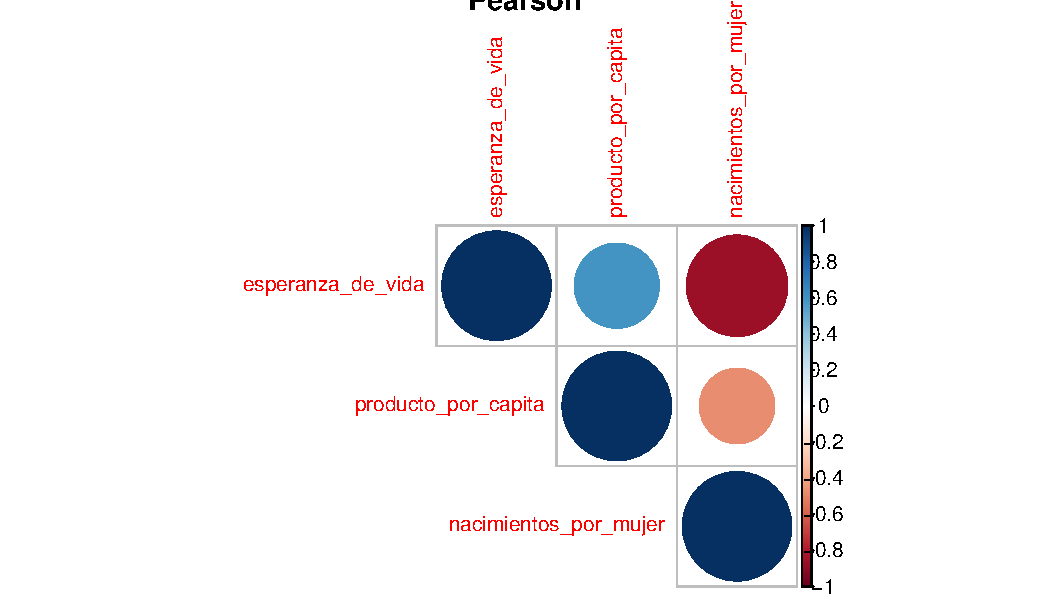
\includegraphics{Informe-del-proyecto._files/figure-latex/unnamed-chunk-5-1.pdf}
Se realiza una prueba de correlación de Pearson y Spearman para
identificar correlaciones positivas como negativas.

\begin{Shaded}
\begin{Highlighting}[]
\CommentTok{\# Filtrar datos si deseas hacerlo por año específico (opcional)}
\NormalTok{datos\_filtrados }\OtherTok{\textless{}{-}}\NormalTok{ Datos\_FEGDP }\SpecialCharTok{\%\textgreater{}\%} \FunctionTok{filter}\NormalTok{(year }\SpecialCharTok{==} \DecValTok{2000}\NormalTok{)}

\CommentTok{\# Seleccionar solo las variables numéricas de interés}
\NormalTok{variables }\OtherTok{\textless{}{-}}\NormalTok{ datos\_filtrados }\SpecialCharTok{\%\textgreater{}\%}
  \FunctionTok{select}\NormalTok{(esperanza\_de\_vida, producto\_por\_capita, nacimientos\_por\_mujer)}
\CommentTok{\# Correlación de Pearson}
\NormalTok{cor\_pearson }\OtherTok{\textless{}{-}} \FunctionTok{cor}\NormalTok{(variables, }\AttributeTok{method =} \StringTok{"pearson"}\NormalTok{, }\AttributeTok{use =} \StringTok{"complete.obs"}\NormalTok{)}

\CommentTok{\# Correlación de Spearman}
\NormalTok{cor\_spearman }\OtherTok{\textless{}{-}} \FunctionTok{cor}\NormalTok{(variables, }\AttributeTok{method =} \StringTok{"spearman"}\NormalTok{, }\AttributeTok{use =} \StringTok{"complete.obs"}\NormalTok{)}

\CommentTok{\# Mostrar resultados}
\FunctionTok{print}\NormalTok{(}\StringTok{"Correlación de Pearson:"}\NormalTok{)}
\end{Highlighting}
\end{Shaded}

\begin{verbatim}
## [1] "Correlación de Pearson:"
\end{verbatim}

\begin{Shaded}
\begin{Highlighting}[]
\FunctionTok{print}\NormalTok{(}\FunctionTok{round}\NormalTok{(cor\_pearson, }\DecValTok{3}\NormalTok{))}
\end{Highlighting}
\end{Shaded}

\begin{verbatim}
##                       esperanza_de_vida producto_por_capita
## esperanza_de_vida                 1.000                0.60
## producto_por_capita               0.600                1.00
## nacimientos_por_mujer            -0.856               -0.47
##                       nacimientos_por_mujer
## esperanza_de_vida                    -0.856
## producto_por_capita                  -0.470
## nacimientos_por_mujer                 1.000
\end{verbatim}

\begin{Shaded}
\begin{Highlighting}[]
\FunctionTok{print}\NormalTok{(}\StringTok{"Correlación de Spearman:"}\NormalTok{)}
\end{Highlighting}
\end{Shaded}

\begin{verbatim}
## [1] "Correlación de Spearman:"
\end{verbatim}

\begin{Shaded}
\begin{Highlighting}[]
\FunctionTok{print}\NormalTok{(}\FunctionTok{round}\NormalTok{(cor\_spearman, }\DecValTok{3}\NormalTok{))}
\end{Highlighting}
\end{Shaded}

\begin{verbatim}
##                       esperanza_de_vida producto_por_capita
## esperanza_de_vida                 1.000               0.870
## producto_por_capita               0.870               1.000
## nacimientos_por_mujer            -0.823              -0.742
##                       nacimientos_por_mujer
## esperanza_de_vida                    -0.823
## producto_por_capita                  -0.742
## nacimientos_por_mujer                 1.000
\end{verbatim}

Tanto en los gráficos generales como en las pruebas se puede ver que hay
una correlación positiva entre esperanza de vida y PIB, mientras que hay
una negativa entre esperanza de vida y fecundidad, lo mismo que se puede
ver en los gráficos, a su vez, también se puede ver una correlación
negativa entre el PIB per cápita y la fecundidad.

\begin{Shaded}
\begin{Highlighting}[]
\CommentTok{\# Visualizar matriz de Pearson}
\FunctionTok{corrplot}\NormalTok{(cor\_pearson, }\AttributeTok{method =} \StringTok{"circle"}\NormalTok{, }\AttributeTok{type =} \StringTok{"upper"}\NormalTok{, }\AttributeTok{tl.cex =} \FloatTok{0.8}\NormalTok{, }\AttributeTok{title =} \StringTok{"Pearson"}\NormalTok{)}
\end{Highlighting}
\end{Shaded}

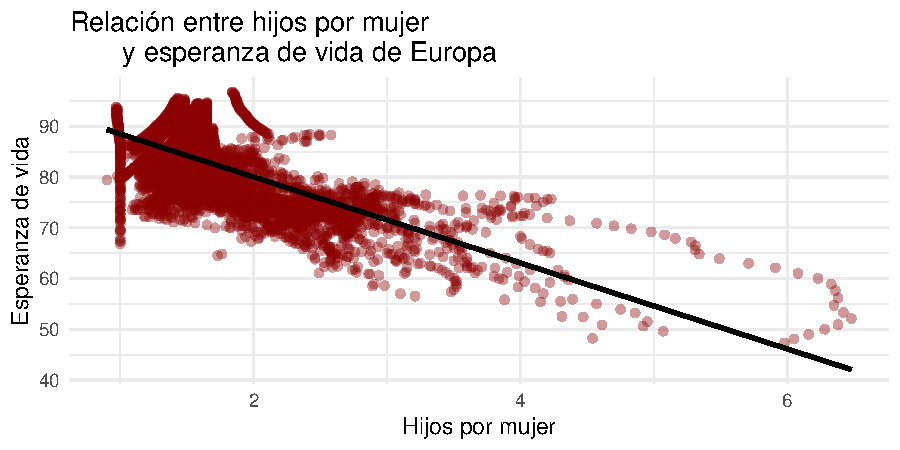
\includegraphics{Informe-del-proyecto._files/figure-latex/unnamed-chunk-7-1.pdf}

\begin{Shaded}
\begin{Highlighting}[]
\CommentTok{\# Visualizar matriz de Spearman}
\FunctionTok{corrplot}\NormalTok{(cor\_spearman, }\AttributeTok{method =} \StringTok{"circle"}\NormalTok{, }\AttributeTok{type =} \StringTok{"upper"}\NormalTok{, }\AttributeTok{tl.cex =} \FloatTok{0.8}\NormalTok{, }\AttributeTok{title =} \StringTok{"Spearman"}\NormalTok{)}
\end{Highlighting}
\end{Shaded}

\includegraphics{Informe-del-proyecto._files/figure-latex/unnamed-chunk-7-2.pdf}
Los resultados respaldan los patrones visuales observados anteriormente
mediante gráficos.

\textbf{Análisis Regional}

Europa presenta un comportamiento particular: Se observa una caída en la
cantidad de hijos por mujeres y con esto también la esperanza de vida en
países con 2 hijos por mujer, aunque no se trata de una reducción
sistemática. De hecho, varios países con solo 1 hijo muestran menor
esperanza de vida que aquellos con 2, lo cual podría deberse a factores
contextuales como el envejecimiento poblacional o las políticas de
salud.

\begin{Shaded}
\begin{Highlighting}[]
\NormalTok{datos\_filtrados }\OtherTok{\textless{}{-}}\NormalTok{ Datos\_FEGDP }\SpecialCharTok{\%\textgreater{}\%}
  \FunctionTok{filter}\NormalTok{(continente }\SpecialCharTok{==} \StringTok{"Europe"}\NormalTok{)}
  
\FunctionTok{ggplot}\NormalTok{(datos\_filtrados, }\FunctionTok{aes}\NormalTok{(}\AttributeTok{x =}\NormalTok{ nacimientos\_por\_mujer, }\AttributeTok{y =}\NormalTok{ esperanza\_de\_vida)) }\SpecialCharTok{+}
  \FunctionTok{geom\_point}\NormalTok{(}\AttributeTok{alpha =} \FloatTok{0.4}\NormalTok{, }\AttributeTok{color =} \StringTok{"darkred"}\NormalTok{) }\SpecialCharTok{+}
  \FunctionTok{geom\_smooth}\NormalTok{(}\AttributeTok{method =} \StringTok{"lm"}\NormalTok{, }\AttributeTok{se =} \ConstantTok{FALSE}\NormalTok{, }\AttributeTok{color =} \StringTok{"black"}\NormalTok{) }\SpecialCharTok{+}
  \FunctionTok{labs}\NormalTok{(}\AttributeTok{title =} \StringTok{"Relación entre hijos por mujer }
\StringTok{       y esperanza de vida de Europa"}\NormalTok{, }\AttributeTok{x =} \StringTok{"Hijos por mujer"}\NormalTok{, }\AttributeTok{y =} \StringTok{"Esperanza de vida"}\NormalTok{) }\SpecialCharTok{+}
  \FunctionTok{theme\_minimal}\NormalTok{()}
\end{Highlighting}
\end{Shaded}

\begin{verbatim}
## `geom_smooth()` using formula = 'y ~ x'
\end{verbatim}

\begin{verbatim}
## Warning: Removed 906 rows containing non-finite outside the scale range
## (`stat_smooth()`).
\end{verbatim}

\begin{verbatim}
## Warning: Removed 906 rows containing missing values or values outside the scale range
## (`geom_point()`).
\end{verbatim}

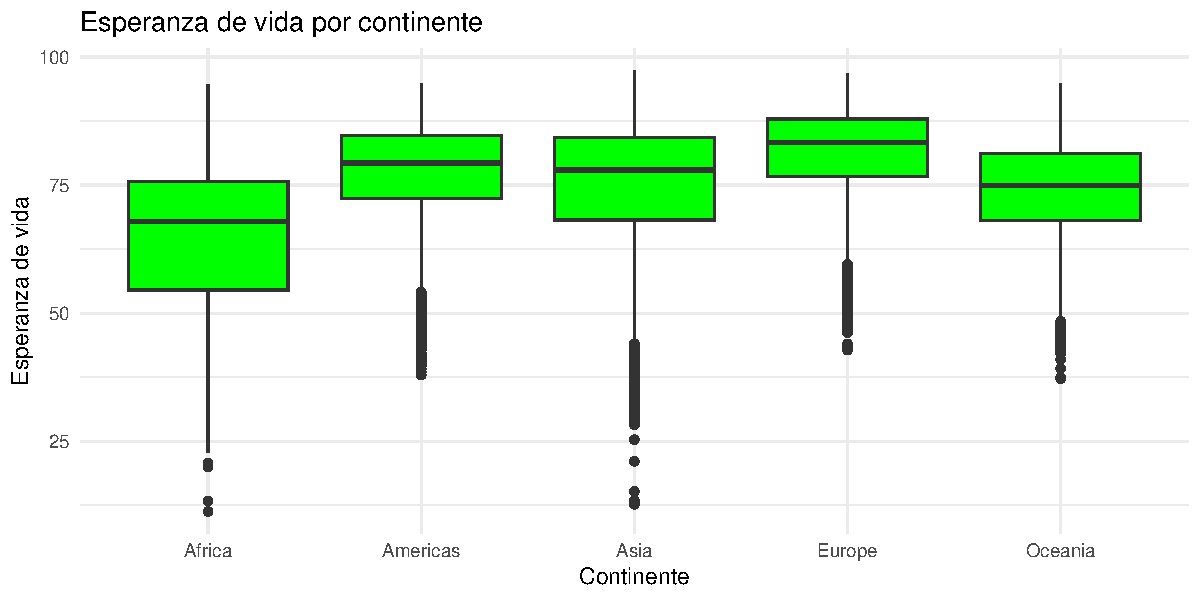
\includegraphics{Informe-del-proyecto._files/figure-latex/unnamed-chunk-8-1.pdf}

En el caso de África, se registra la esperanza de vida más baja en
comparación con otros continentes, manteniéndose la tendencia
decreciente a pesar de una alta fecundidad.

\begin{Shaded}
\begin{Highlighting}[]
\FunctionTok{ggplot}\NormalTok{(Datos\_FEGDP, }\FunctionTok{aes}\NormalTok{(}\AttributeTok{x =}\NormalTok{ continente, }\AttributeTok{y =}\NormalTok{ esperanza\_de\_vida)) }\SpecialCharTok{+}
  \FunctionTok{geom\_boxplot}\NormalTok{(}\AttributeTok{fill =} \StringTok{"green"}\NormalTok{) }\SpecialCharTok{+}
  \FunctionTok{labs}\NormalTok{(}\AttributeTok{title =} \StringTok{"Esperanza de vida por continente"}\NormalTok{, }\AttributeTok{y =} \StringTok{"Esperanza de vida"}\NormalTok{, }\AttributeTok{x =} \StringTok{"Continente"}\NormalTok{) }\SpecialCharTok{+}
  \FunctionTok{theme\_minimal}\NormalTok{()}
\end{Highlighting}
\end{Shaded}

\begin{verbatim}
## Warning: Removed 5 rows containing non-finite outside the scale range
## (`stat_boxplot()`).
\end{verbatim}

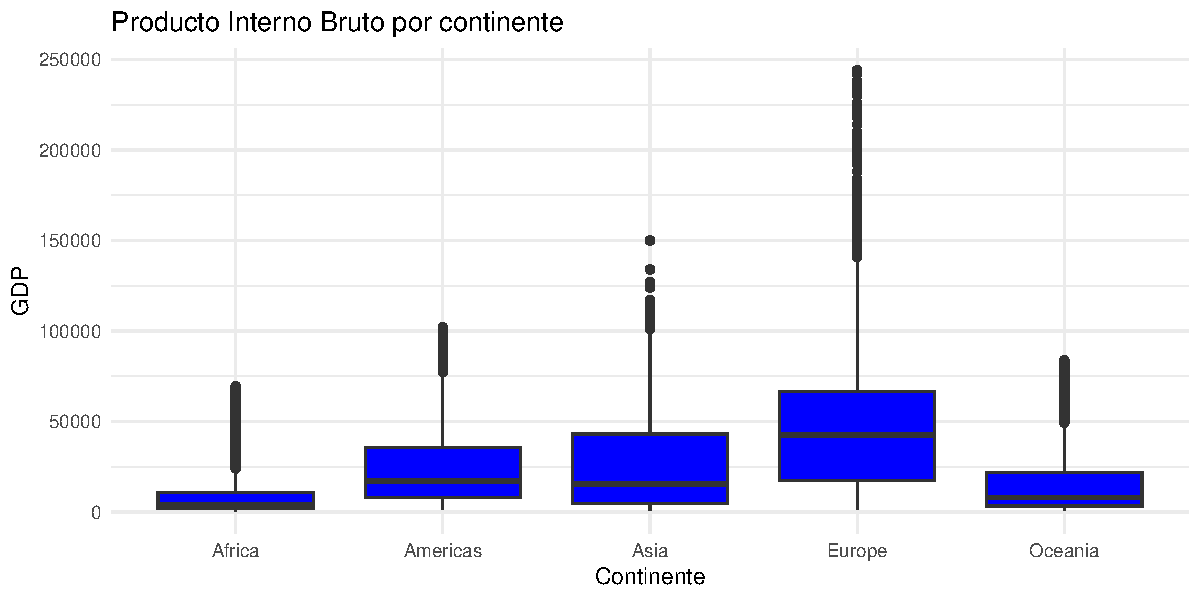
\includegraphics{Informe-del-proyecto._files/figure-latex/unnamed-chunk-9-1.pdf}
Continuando con la misma región, el bajo nivel del PIB per cápita
también resalta como un elemento que podría influir en los resultados,
reflejando bajos niveles de desarrollo económico.

\begin{Shaded}
\begin{Highlighting}[]
\FunctionTok{ggplot}\NormalTok{(Datos\_FEGDP, }\FunctionTok{aes}\NormalTok{(}\AttributeTok{x =}\NormalTok{ continente, }\AttributeTok{y =}\NormalTok{ producto\_por\_capita)) }\SpecialCharTok{+}
  \FunctionTok{geom\_boxplot}\NormalTok{(}\AttributeTok{fill =} \StringTok{"blue"}\NormalTok{) }\SpecialCharTok{+}
  \FunctionTok{labs}\NormalTok{(}\AttributeTok{title =} \StringTok{"Producto Interno Bruto por continente"}\NormalTok{, }\AttributeTok{y =} \StringTok{"GDP"}\NormalTok{, }\AttributeTok{x =} \StringTok{"Continente"}\NormalTok{) }\SpecialCharTok{+}
  \FunctionTok{theme\_minimal}\NormalTok{()}
\end{Highlighting}
\end{Shaded}

\begin{verbatim}
## Warning: Removed 7550 rows containing non-finite outside the scale range
## (`stat_boxplot()`).
\end{verbatim}

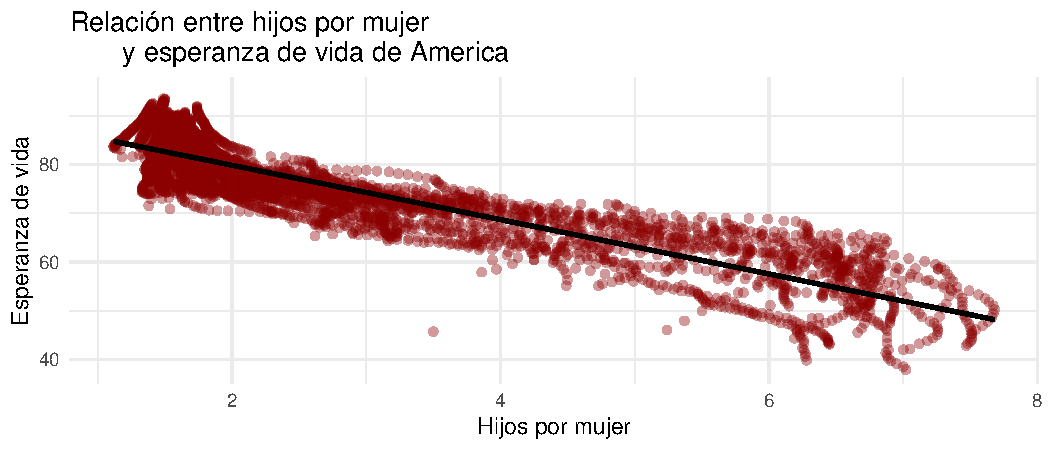
\includegraphics{Informe-del-proyecto._files/figure-latex/unnamed-chunk-10-1.pdf}

En las Américas, se conserva la tendencia general: los países con mayor
fecundidad tienden a registrar niveles más bajos de esperanza de vida.
Este patrón refuerza la hipótesis de una correlación negativa entre
estas dos variables, aunque no necesariamente causal.

\begin{Shaded}
\begin{Highlighting}[]
\NormalTok{datos\_filtrados }\OtherTok{\textless{}{-}}\NormalTok{ Datos\_FEGDP }\SpecialCharTok{\%\textgreater{}\%}
  \FunctionTok{filter}\NormalTok{(continente }\SpecialCharTok{==} \StringTok{"Americas"}\NormalTok{)}
  
\FunctionTok{ggplot}\NormalTok{(datos\_filtrados, }\FunctionTok{aes}\NormalTok{(}\AttributeTok{x =}\NormalTok{ nacimientos\_por\_mujer, }\AttributeTok{y =}\NormalTok{ esperanza\_de\_vida)) }\SpecialCharTok{+}
  \FunctionTok{geom\_point}\NormalTok{(}\AttributeTok{alpha =} \FloatTok{0.4}\NormalTok{, }\AttributeTok{color =} \StringTok{"darkred"}\NormalTok{) }\SpecialCharTok{+}
  \FunctionTok{geom\_smooth}\NormalTok{(}\AttributeTok{method =} \StringTok{"lm"}\NormalTok{, }\AttributeTok{se =} \ConstantTok{FALSE}\NormalTok{, }\AttributeTok{color =} \StringTok{"black"}\NormalTok{) }\SpecialCharTok{+}
  \FunctionTok{labs}\NormalTok{(}\AttributeTok{title =} \StringTok{"Relación entre hijos por mujer }
\StringTok{       y esperanza de vida de America"}\NormalTok{, }\AttributeTok{x =} \StringTok{"Hijos por mujer"}\NormalTok{, }\AttributeTok{y =} \StringTok{"Esperanza de vida"}\NormalTok{) }\SpecialCharTok{+}
  \FunctionTok{theme\_minimal}\NormalTok{()}
\end{Highlighting}
\end{Shaded}

\begin{verbatim}
## `geom_smooth()` using formula = 'y ~ x'
\end{verbatim}

\begin{verbatim}
## Warning: Removed 2869 rows containing non-finite outside the scale range
## (`stat_smooth()`).
\end{verbatim}

\begin{verbatim}
## Warning: Removed 2869 rows containing missing values or values outside the scale range
## (`geom_point()`).
\end{verbatim}

\includegraphics{Informe-del-proyecto._files/figure-latex/unnamed-chunk-11-1.pdf}
En la sección de gráficos de interacción avanzada, se identifican
valores altos de esperanza de vida asociados a tasas de fecundidad
cercanas a 0.7 hijos por mujer, con una esperanza de vida promedio entre
86 y 89 años.

\begin{Shaded}
\begin{Highlighting}[]
\NormalTok{vida\_min }\OtherTok{\textless{}{-}} \DecValTok{86}
\NormalTok{vida\_max }\OtherTok{\textless{}{-}} \DecValTok{89}
  
  \CommentTok{\# Filtrar datos según los inputs}
\NormalTok{  datos\_filtrados }\OtherTok{\textless{}{-}}\NormalTok{ Datos\_FEGDP }\SpecialCharTok{\%\textgreater{}\%}
    \FunctionTok{filter}\NormalTok{(}\SpecialCharTok{!}\FunctionTok{is.na}\NormalTok{(nacimientos\_por\_mujer),}
      \SpecialCharTok{!}\FunctionTok{is.na}\NormalTok{(esperanza\_de\_vida)}
\NormalTok{    ) }\SpecialCharTok{\%\textgreater{}\%}
    \FunctionTok{filter}\NormalTok{(esperanza\_de\_vida }\SpecialCharTok{\textgreater{}=}\NormalTok{ vida\_min }\SpecialCharTok{\&}\NormalTok{ esperanza\_de\_vida }\SpecialCharTok{\textless{}=}\NormalTok{ vida\_max)}

\CommentTok{\#Gráfico}
 \FunctionTok{ggplot}\NormalTok{(Datos\_FEGDP, }\FunctionTok{aes}\NormalTok{(}\AttributeTok{x =}\NormalTok{ esperanza\_de\_vida, }\AttributeTok{y =}\NormalTok{ nacimientos\_por\_mujer)) }\SpecialCharTok{+}
    \FunctionTok{geom\_point}\NormalTok{(}\AttributeTok{alpha =} \FloatTok{0.3}\NormalTok{, }\AttributeTok{color =} \StringTok{"pink"}\NormalTok{) }\SpecialCharTok{+}
    \FunctionTok{geom\_point}\NormalTok{(}\AttributeTok{data =}\NormalTok{ datos\_filtrados, }\FunctionTok{aes}\NormalTok{(}\AttributeTok{x =}\NormalTok{ esperanza\_de\_vida, }\AttributeTok{y =}\NormalTok{ nacimientos\_por\_mujer), }
               \AttributeTok{color =} \StringTok{"blue"}\NormalTok{, }\AttributeTok{size =} \DecValTok{3}\NormalTok{) }\SpecialCharTok{+}
    \FunctionTok{geom\_smooth}\NormalTok{(}\AttributeTok{method =} \StringTok{"loess"}\NormalTok{, }\AttributeTok{se =} \ConstantTok{FALSE}\NormalTok{, }\AttributeTok{color =} \StringTok{"black"}\NormalTok{) }\SpecialCharTok{+}
    \FunctionTok{labs}\NormalTok{(}
      \AttributeTok{title =} \FunctionTok{paste}\NormalTok{(}\StringTok{"Hijos por mujer según esperanza de vida"}\NormalTok{,}
\NormalTok{                    vida\_min, }\StringTok{"y"}\NormalTok{, vida\_max, }\StringTok{"años"}\NormalTok{),}
      \AttributeTok{x =} \StringTok{"Esperanza de vida (años)"}\NormalTok{,}
      \AttributeTok{y =} \StringTok{"Hijos por mujer"}
\NormalTok{    ) }\SpecialCharTok{+}
    \FunctionTok{theme\_minimal}\NormalTok{()}
\end{Highlighting}
\end{Shaded}

\begin{verbatim}
## `geom_smooth()` using formula = 'y ~ x'
\end{verbatim}

\begin{verbatim}
## Warning: Removed 5893 rows containing non-finite outside the scale range
## (`stat_smooth()`).
\end{verbatim}

\begin{verbatim}
## Warning: Removed 5893 rows containing missing values or values outside the scale range
## (`geom_point()`).
\end{verbatim}

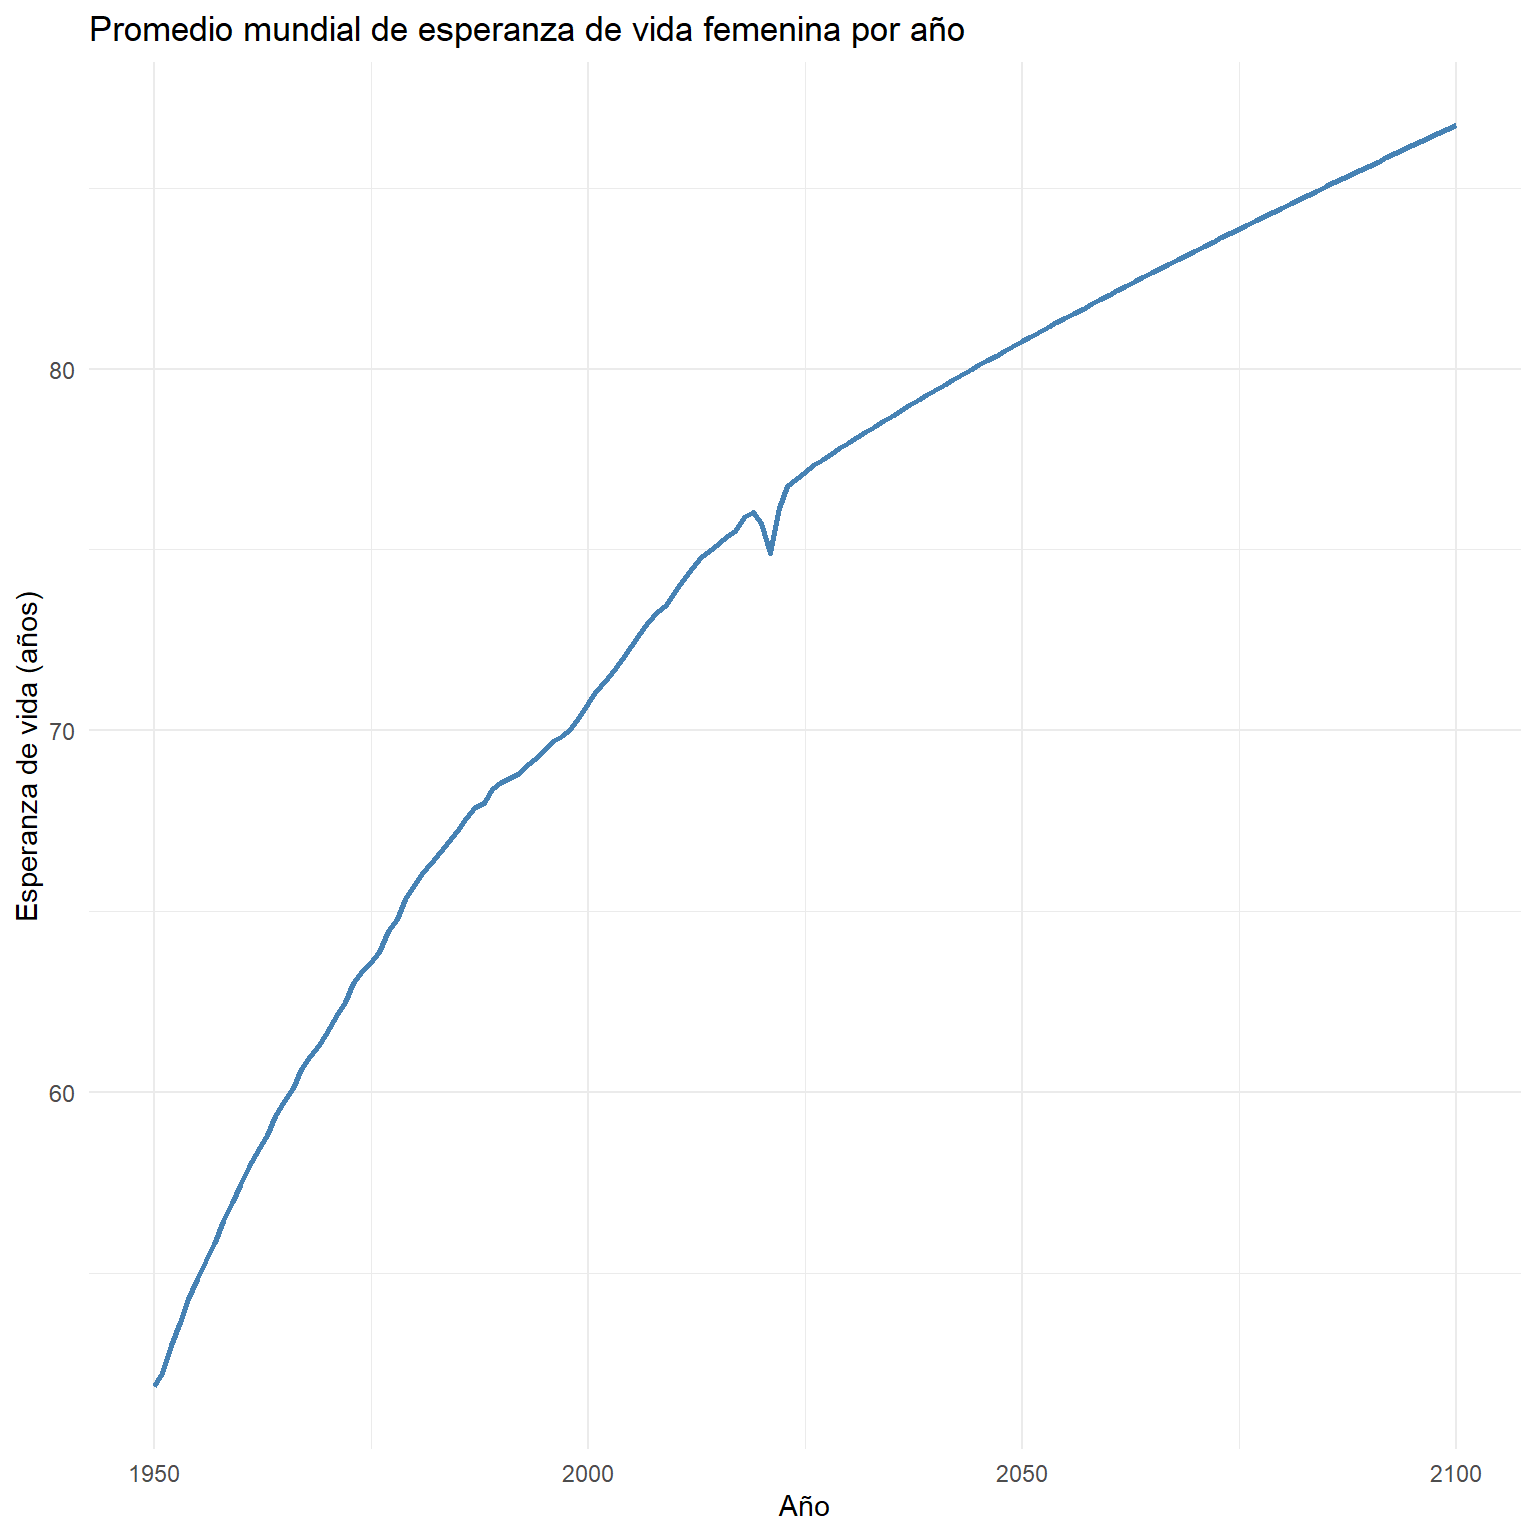
\includegraphics{Informe-del-proyecto._files/figure-latex/unnamed-chunk-12-1.pdf}

Por otro lado, los países con una fecundidad de 1 hijo muestran una
esperanza de vida aún mayor, entre 93 y 96 años. Esto sugiere que los
países con baja fecundidad tienden a presentar mayores niveles de
longevidad. Sin embargo, no se observa un patrón lineal estricto: no
puede afirmarse que a menor número de hijos por mujer siempre
corresponda una mayor esperanza de vida.

\begin{Shaded}
\begin{Highlighting}[]
\NormalTok{vida\_min1 }\OtherTok{\textless{}{-}} \DecValTok{93}
\NormalTok{vida\_max2 }\OtherTok{\textless{}{-}} \DecValTok{96}
  
  \CommentTok{\# Filtrar datos según los inputs}
\NormalTok{  datos\_filtrados }\OtherTok{\textless{}{-}}\NormalTok{ Datos\_FEGDP }\SpecialCharTok{\%\textgreater{}\%}
    \FunctionTok{filter}\NormalTok{(}\SpecialCharTok{!}\FunctionTok{is.na}\NormalTok{(nacimientos\_por\_mujer),}
      \SpecialCharTok{!}\FunctionTok{is.na}\NormalTok{(esperanza\_de\_vida)}
\NormalTok{    ) }\SpecialCharTok{\%\textgreater{}\%}
    \FunctionTok{filter}\NormalTok{(esperanza\_de\_vida }\SpecialCharTok{\textgreater{}=}\NormalTok{ vida\_min1 }\SpecialCharTok{\&}\NormalTok{ esperanza\_de\_vida }\SpecialCharTok{\textless{}=}\NormalTok{ vida\_max2)}

\CommentTok{\#Gráfico}
 \FunctionTok{ggplot}\NormalTok{(Datos\_FEGDP, }\FunctionTok{aes}\NormalTok{(}\AttributeTok{x =}\NormalTok{ esperanza\_de\_vida, }\AttributeTok{y =}\NormalTok{ nacimientos\_por\_mujer)) }\SpecialCharTok{+}
    \FunctionTok{geom\_point}\NormalTok{(}\AttributeTok{alpha =} \FloatTok{0.3}\NormalTok{, }\AttributeTok{color =} \StringTok{"pink"}\NormalTok{) }\SpecialCharTok{+}
    \FunctionTok{geom\_point}\NormalTok{(}\AttributeTok{data =}\NormalTok{ datos\_filtrados, }\FunctionTok{aes}\NormalTok{(}\AttributeTok{x =}\NormalTok{ esperanza\_de\_vida, }\AttributeTok{y =}\NormalTok{ nacimientos\_por\_mujer), }
               \AttributeTok{color =} \StringTok{"blue"}\NormalTok{, }\AttributeTok{size =} \DecValTok{3}\NormalTok{) }\SpecialCharTok{+}
    \FunctionTok{geom\_smooth}\NormalTok{(}\AttributeTok{method =} \StringTok{"loess"}\NormalTok{, }\AttributeTok{se =} \ConstantTok{FALSE}\NormalTok{, }\AttributeTok{color =} \StringTok{"black"}\NormalTok{) }\SpecialCharTok{+}
    \FunctionTok{labs}\NormalTok{(}
      \AttributeTok{title =} \FunctionTok{paste}\NormalTok{(}\StringTok{"Hijos por mujer según esperanza de vida"}\NormalTok{,}
\NormalTok{                    vida\_min1, }\StringTok{"y"}\NormalTok{, vida\_max2, }\StringTok{"años"}\NormalTok{),}
      \AttributeTok{x =} \StringTok{"Esperanza de vida (años)"}\NormalTok{,}
      \AttributeTok{y =} \StringTok{"Hijos por mujer"}
\NormalTok{    ) }\SpecialCharTok{+}
    \FunctionTok{theme\_minimal}\NormalTok{()}
\end{Highlighting}
\end{Shaded}

\begin{verbatim}
## `geom_smooth()` using formula = 'y ~ x'
\end{verbatim}

\begin{verbatim}
## Warning: Removed 5893 rows containing non-finite outside the scale range
## (`stat_smooth()`).
\end{verbatim}

\begin{verbatim}
## Warning: Removed 5893 rows containing missing values or values outside the scale range
## (`geom_point()`).
\end{verbatim}

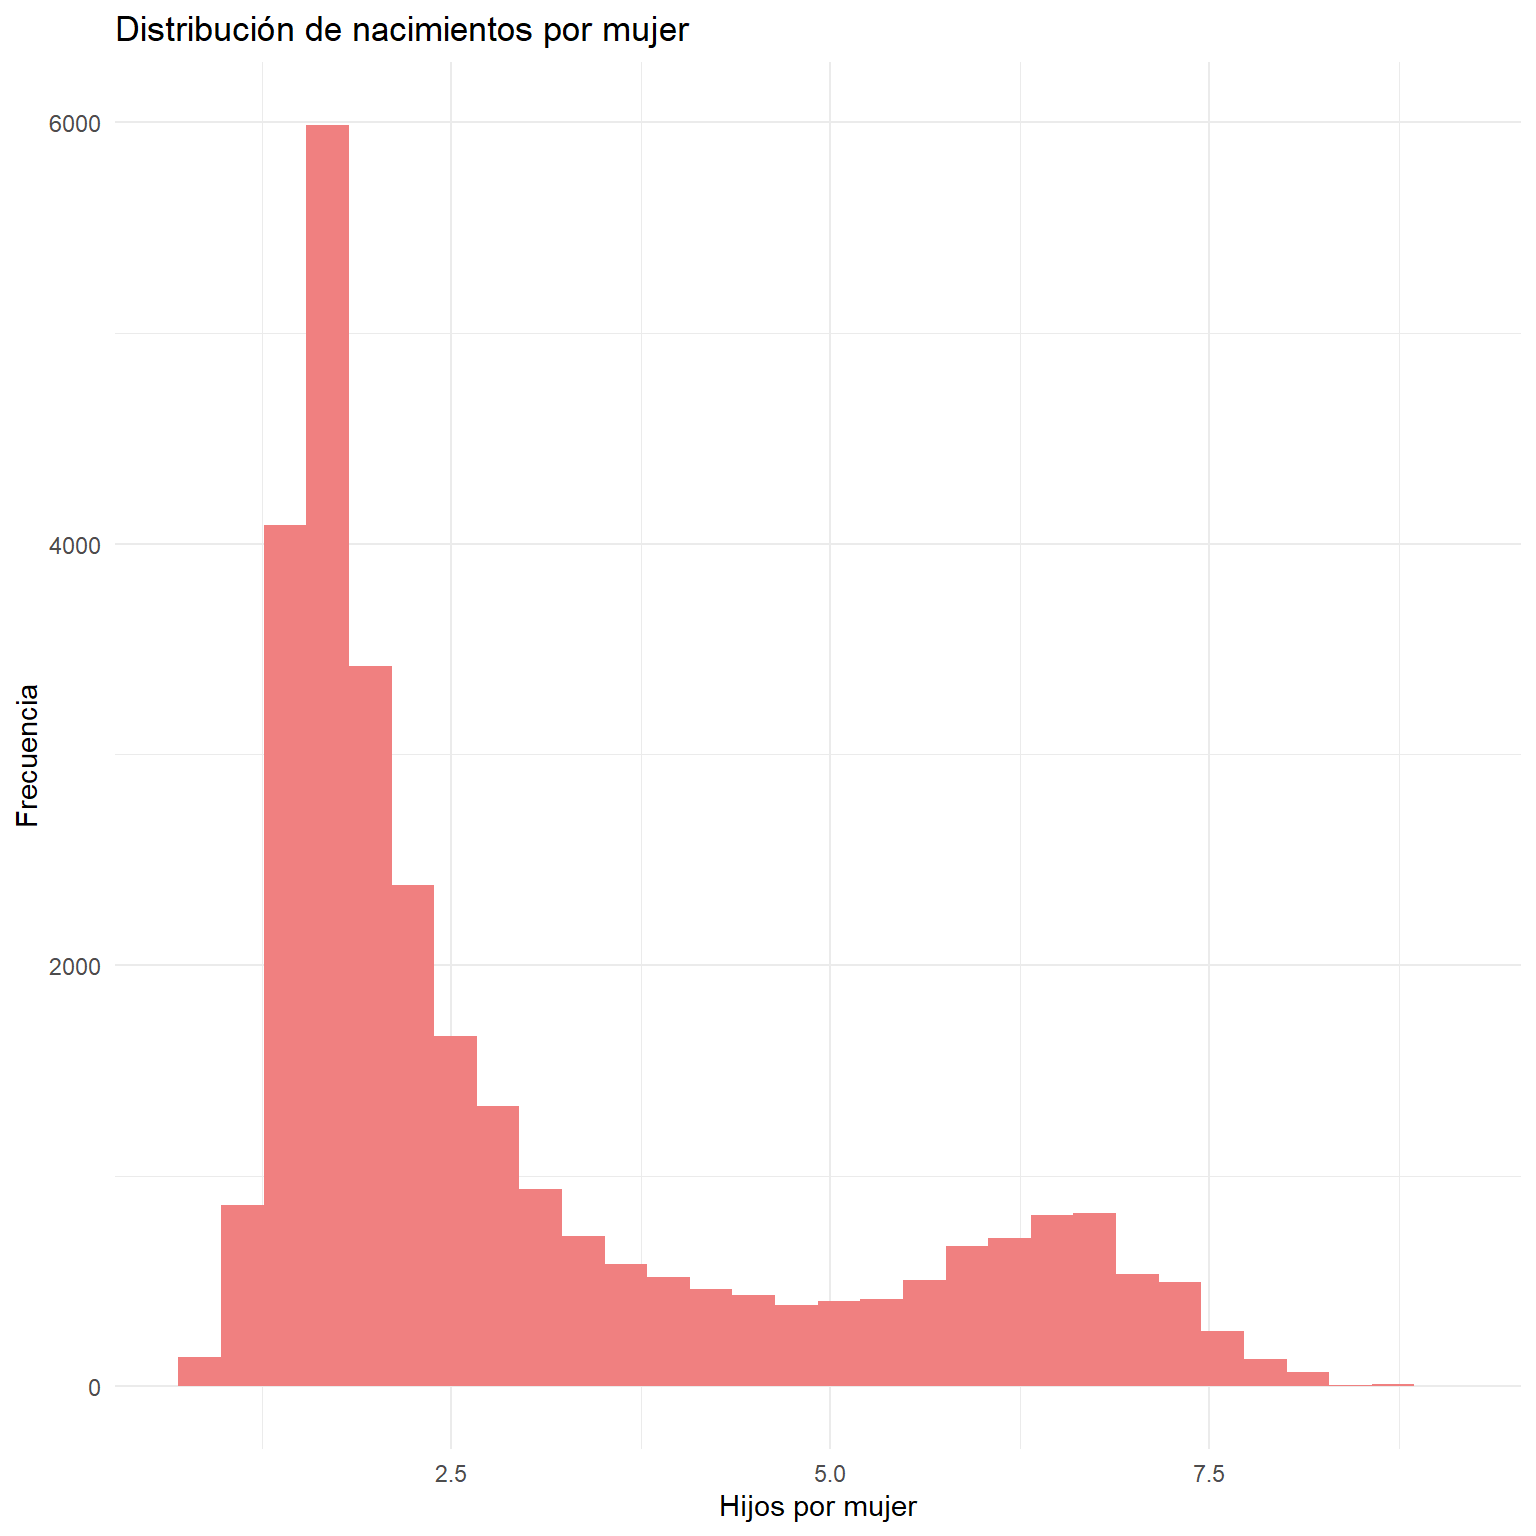
\includegraphics{Informe-del-proyecto._files/figure-latex/unnamed-chunk-13-1.pdf}

Aunque no se puede concluir que tener hijos necesariamente alarga o
acorta la vida, los gráficos permiten identificar tendencias
consistentes, especialmente al analizar los datos por regiones o niveles
de desarrollo económico.

En cuanto al PIB per cápita, el gráfico de interacción avanzada muestra
cómo esta variable se asocia tanto con fecundidad como con esperanza de
vida. En el gráfico ``Relación entre GDP, fecundidad y esperanza de
vida'', se observa que los países con PIB superiores a 100,000 dólares
se ubican principalmente en la franja de 2 a 2.5 hijos por mujer, y
presentan una esperanza de vida alta (representada en color azul). Esto
evidencia que, si bien la baja fecundidad puede asociarse con mayor
longevidad, el nivel de desarrollo económico es un factor modulador
clave.

\begin{Shaded}
\begin{Highlighting}[]
\NormalTok{  datos\_filtrados }\OtherTok{\textless{}{-}}\NormalTok{ Datos\_FEGDP }\SpecialCharTok{\%\textgreater{}\%}
    \FunctionTok{filter}\NormalTok{(}
      \SpecialCharTok{!}\FunctionTok{is.na}\NormalTok{(producto\_por\_capita), }
      \SpecialCharTok{!}\FunctionTok{is.na}\NormalTok{(nacimientos\_por\_mujer), }
      \SpecialCharTok{!}\FunctionTok{is.na}\NormalTok{(esperanza\_de\_vida)}
\NormalTok{)}

\CommentTok{\# Gráfico}
\FunctionTok{ggplot}\NormalTok{(datos\_filtrados, }\FunctionTok{aes}\NormalTok{(}\AttributeTok{x =}\NormalTok{ producto\_por\_capita, }
                            \AttributeTok{y =}\NormalTok{ nacimientos\_por\_mujer, }
                            \AttributeTok{size =}\NormalTok{ esperanza\_de\_vida, }
                            \AttributeTok{color =}\NormalTok{ esperanza\_de\_vida)) }\SpecialCharTok{+}
  \FunctionTok{geom\_point}\NormalTok{(}\AttributeTok{alpha =} \FloatTok{0.8}\NormalTok{) }\SpecialCharTok{+}
  \FunctionTok{scale\_x\_log10}\NormalTok{(}\AttributeTok{labels =} \FunctionTok{dollar\_format}\NormalTok{(}\AttributeTok{prefix =} \StringTok{"$"}\NormalTok{)) }\SpecialCharTok{+}
  \FunctionTok{scale\_color\_gradient}\NormalTok{(}\AttributeTok{low =} \StringTok{"red"}\NormalTok{, }\AttributeTok{high =} \StringTok{"blue"}\NormalTok{) }\SpecialCharTok{+}
  \FunctionTok{labs}\NormalTok{(}\AttributeTok{title =} \StringTok{"Relación entre GDP, fecundidad y esperanza de vida"}\NormalTok{,}
       \AttributeTok{x =} \StringTok{"Producto Interno Bruto per cápita (log)"}\NormalTok{,}
       \AttributeTok{y =} \StringTok{"Hijos por mujer"}\NormalTok{,}
       \AttributeTok{color =} \StringTok{"Esperanza de vida (años)"}\NormalTok{,}
       \AttributeTok{size =} \StringTok{"Esperanza de vida"}\NormalTok{) }\SpecialCharTok{+}
  \FunctionTok{theme\_minimal}\NormalTok{()}\SpecialCharTok{+}
  \FunctionTok{theme}\NormalTok{(}
    \AttributeTok{plot.title =} \FunctionTok{element\_text}\NormalTok{(}\AttributeTok{size =} \DecValTok{15}\NormalTok{, }\AttributeTok{face =} \StringTok{"bold"}\NormalTok{),}
    \AttributeTok{axis.title =} \FunctionTok{element\_text}\NormalTok{(}\AttributeTok{size =} \DecValTok{10}\NormalTok{)}
\NormalTok{  )}
\end{Highlighting}
\end{Shaded}

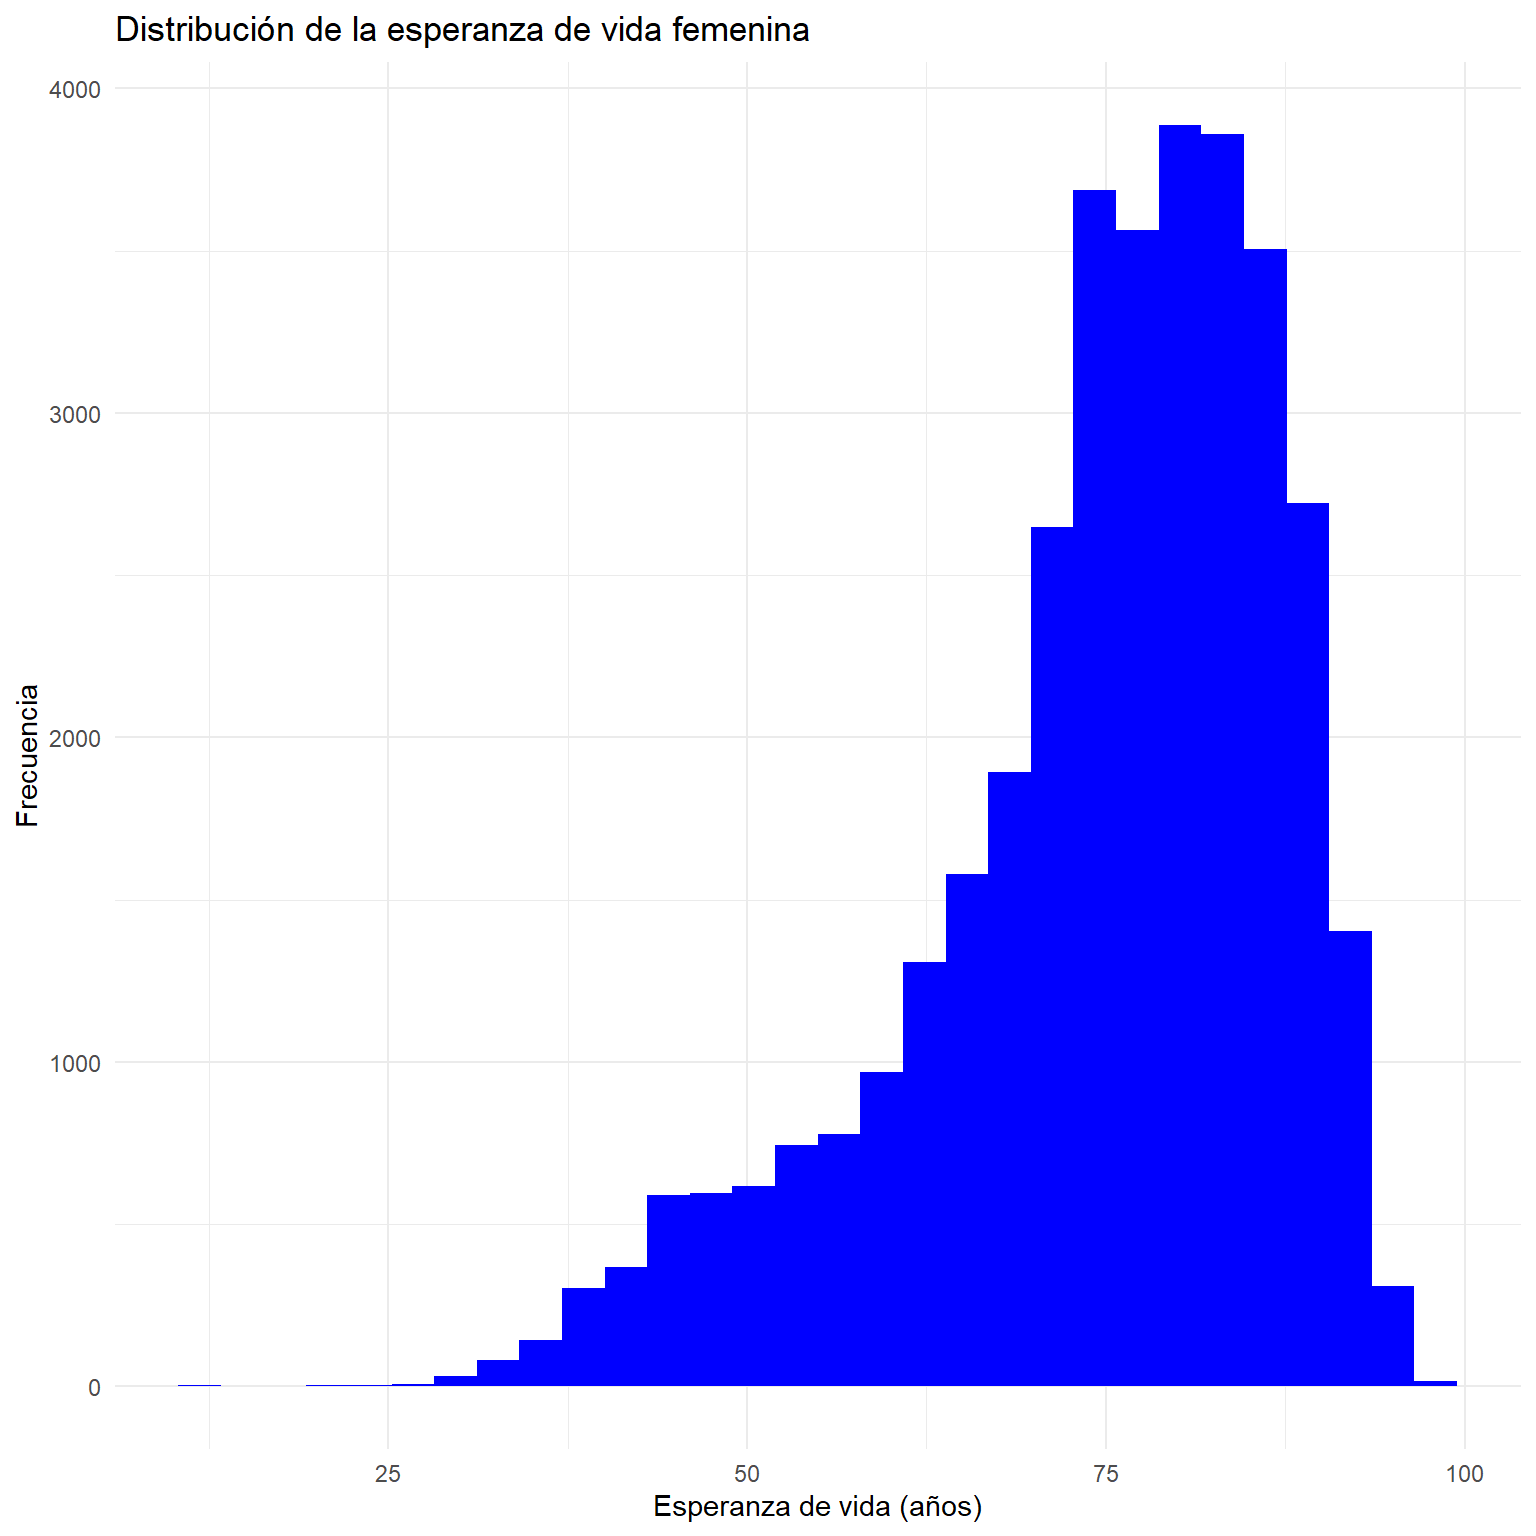
\includegraphics{Informe-del-proyecto._files/figure-latex/unnamed-chunk-14-1.pdf}

Al comparar países según sus niveles de ingreso, se observa que en
aquellos con mayor PIB per cápita, la relación entre baja fecundidad y
alta esperanza de vida es más clara y estable. En contraste, los países
con ingresos bajos presentan relaciones más dispersas, posiblemente
influenciadas por factores externos como conflictos, pobreza estructural
o debilidad institucional.

En cuanto al eje temporal, en el gráfico ``Relación entre GDP,
fecundidad y esperanza de vida'', se aprecia que en 1970 la esperanza de
vida promedio mundial rondaba los 80 años.

\begin{Shaded}
\begin{Highlighting}[]
\NormalTok{  datos\_filtrados }\OtherTok{\textless{}{-}}\NormalTok{ Datos\_FEGDP }\SpecialCharTok{\%\textgreater{}\%}
    \FunctionTok{filter}\NormalTok{( year }\SpecialCharTok{==} \DecValTok{1970}\NormalTok{,}
      \SpecialCharTok{!}\FunctionTok{is.na}\NormalTok{(producto\_por\_capita), }
      \SpecialCharTok{!}\FunctionTok{is.na}\NormalTok{(nacimientos\_por\_mujer), }
      \SpecialCharTok{!}\FunctionTok{is.na}\NormalTok{(esperanza\_de\_vida)}
\NormalTok{)}

\CommentTok{\# Gráfico}
\FunctionTok{ggplot}\NormalTok{(datos\_filtrados, }\FunctionTok{aes}\NormalTok{(}\AttributeTok{x =}\NormalTok{ producto\_por\_capita, }
                            \AttributeTok{y =}\NormalTok{ nacimientos\_por\_mujer, }
                            \AttributeTok{size =}\NormalTok{ esperanza\_de\_vida, }
                            \AttributeTok{color =}\NormalTok{ esperanza\_de\_vida)) }\SpecialCharTok{+}
  \FunctionTok{geom\_point}\NormalTok{(}\AttributeTok{alpha =} \FloatTok{0.8}\NormalTok{) }\SpecialCharTok{+}
  \FunctionTok{scale\_x\_log10}\NormalTok{(}\AttributeTok{labels =} \FunctionTok{dollar\_format}\NormalTok{(}\AttributeTok{prefix =} \StringTok{"$"}\NormalTok{)) }\SpecialCharTok{+}
  \FunctionTok{scale\_color\_gradient}\NormalTok{(}\AttributeTok{low =} \StringTok{"red"}\NormalTok{, }\AttributeTok{high =} \StringTok{"blue"}\NormalTok{) }\SpecialCharTok{+}
  \FunctionTok{labs}\NormalTok{(}\AttributeTok{title =} \StringTok{"Relación entre GDP, fecundidad y esperanza de vida en 1970"}\NormalTok{,}
       \AttributeTok{x =} \StringTok{"Producto Interno Bruto per cápita (log)"}\NormalTok{,}
       \AttributeTok{y =} \StringTok{"Hijos por mujer"}\NormalTok{,}
       \AttributeTok{color =} \StringTok{"Esperanza de vida (años)"}\NormalTok{,}
       \AttributeTok{size =} \StringTok{"Esperanza de vida"}\NormalTok{) }\SpecialCharTok{+}
  \FunctionTok{theme\_minimal}\NormalTok{()}\SpecialCharTok{+}
  \FunctionTok{theme}\NormalTok{(}
    \AttributeTok{plot.title =} \FunctionTok{element\_text}\NormalTok{(}\AttributeTok{size =} \DecValTok{15}\NormalTok{, }\AttributeTok{face =} \StringTok{"bold"}\NormalTok{),}
    \AttributeTok{axis.title =} \FunctionTok{element\_text}\NormalTok{(}\AttributeTok{size =} \DecValTok{10}\NormalTok{)}
\NormalTok{  )}
\end{Highlighting}
\end{Shaded}

\includegraphics{Informe-del-proyecto._files/figure-latex/unnamed-chunk-15-1.pdf}
Para el año 2000, esta cifra aumentó casi en una década, acercándose a
los 90 años. Este incremento evidencia mejoras globales en salud,
condiciones de vida y acceso a servicios básicos.

\begin{Shaded}
\begin{Highlighting}[]
\NormalTok{  datos\_filtrados }\OtherTok{\textless{}{-}}\NormalTok{ Datos\_FEGDP }\SpecialCharTok{\%\textgreater{}\%}
    \FunctionTok{filter}\NormalTok{( year }\SpecialCharTok{==} \DecValTok{2000}\NormalTok{,}
      \SpecialCharTok{!}\FunctionTok{is.na}\NormalTok{(producto\_por\_capita), }
      \SpecialCharTok{!}\FunctionTok{is.na}\NormalTok{(nacimientos\_por\_mujer), }
      \SpecialCharTok{!}\FunctionTok{is.na}\NormalTok{(esperanza\_de\_vida)}
\NormalTok{)}

\CommentTok{\# Gráfico}
\FunctionTok{ggplot}\NormalTok{(datos\_filtrados, }\FunctionTok{aes}\NormalTok{(}\AttributeTok{x =}\NormalTok{ producto\_por\_capita, }
                            \AttributeTok{y =}\NormalTok{ nacimientos\_por\_mujer, }
                            \AttributeTok{size =}\NormalTok{ esperanza\_de\_vida, }
                            \AttributeTok{color =}\NormalTok{ esperanza\_de\_vida)) }\SpecialCharTok{+}
  \FunctionTok{geom\_point}\NormalTok{(}\AttributeTok{alpha =} \FloatTok{0.8}\NormalTok{) }\SpecialCharTok{+}
  \FunctionTok{scale\_x\_log10}\NormalTok{(}\AttributeTok{labels =} \FunctionTok{dollar\_format}\NormalTok{(}\AttributeTok{prefix =} \StringTok{"$"}\NormalTok{)) }\SpecialCharTok{+}
  \FunctionTok{scale\_color\_gradient}\NormalTok{(}\AttributeTok{low =} \StringTok{"red"}\NormalTok{, }\AttributeTok{high =} \StringTok{"blue"}\NormalTok{) }\SpecialCharTok{+}
  \FunctionTok{labs}\NormalTok{(}\AttributeTok{title =} \StringTok{"Relación entre GDP, fecundidad y esperanza de vida en 2000"}\NormalTok{,}
       \AttributeTok{x =} \StringTok{"Producto Interno Bruto per cápita (log)"}\NormalTok{,}
       \AttributeTok{y =} \StringTok{"Hijos por mujer"}\NormalTok{,}
       \AttributeTok{color =} \StringTok{"Esperanza de vida (años)"}\NormalTok{,}
       \AttributeTok{size =} \StringTok{"Esperanza de vida"}\NormalTok{) }\SpecialCharTok{+}
  \FunctionTok{theme\_minimal}\NormalTok{()}\SpecialCharTok{+}
  \FunctionTok{theme}\NormalTok{(}
    \AttributeTok{plot.title =} \FunctionTok{element\_text}\NormalTok{(}\AttributeTok{size =} \DecValTok{15}\NormalTok{, }\AttributeTok{face =} \StringTok{"bold"}\NormalTok{),}
    \AttributeTok{axis.title =} \FunctionTok{element\_text}\NormalTok{(}\AttributeTok{size =} \DecValTok{10}\NormalTok{)}
\NormalTok{  )}
\end{Highlighting}
\end{Shaded}

\includegraphics{Informe-del-proyecto._files/figure-latex/unnamed-chunk-16-1.pdf}

Aunque la fecundidad no constituye un determinante único en la decisión
de tener hijos ni en la esperanza de vida, sí representa un componente
clave en el análisis con perspectiva de género. Las decisiones
reproductivas están profundamente influenciadas por factores sociales,
económicos y culturales, que varían según el contexto y el nivel de
desarrollo.

Además, existen otras perspectivas que no pudieron abordarse en esta
investigación debido a la falta de información disponible, como el rol
del compañero o compañera de crianza, así como la presencia de redes de
apoyo familiares, comunitarias o institucionales. Estos factores pueden
influir significativamente en la experiencia reproductiva, el bienestar
emocional y la salud a largo plazo de las mujeres, y podrían ser
determinantes en la relación entre maternidad y longevidad. Su inclusión
en futuros estudios permitiría ampliar el análisis hacia una comprensión
más integral del contexto en que se toman las decisiones reproductivas y
se vive la maternidad.

En este estudio, la regresión múltiple revela que el PIB per cápita y la
fecundidad explican conjuntamente más del 84\% de la variabilidad en la
esperanza de vida femenina. Este resultado evidencia una correlación
multivariable sólida entre desarrollo económico, salud y dinámica
demográfica, y refuerza la necesidad de abordar los indicadores
poblacionales desde una mirada integrada y contextualizada.

Además, estos hallazgos se alinean con estudios previos que sugieren un
vínculo entre decisiones reproductivas y longevidad femenina. Si bien no
se puede establecer una relación causal directa, los datos apuntan a que
niveles moderados de fecundidad ---como tener un solo hijo--- podrían
asociarse con una mayor esperanza de vida, especialmente en contextos
con mejores condiciones socioeconómicas.

\begin{Shaded}
\begin{Highlighting}[]
\CommentTok{\# Modelo de regresión múltiple}
\NormalTok{modelo }\OtherTok{\textless{}{-}} \FunctionTok{lm}\NormalTok{(variables, }\AttributeTok{data =}\NormalTok{ Datos\_FEGDP)}

\CommentTok{\# Resumen del modelo}
\FunctionTok{summary}\NormalTok{(modelo)}
\end{Highlighting}
\end{Shaded}

\begin{verbatim}
## 
## Call:
## lm(formula = variables, data = Datos_FEGDP)
## 
## Residuals:
##     Min      1Q  Median      3Q     Max 
## -58.855  -2.576   0.313   3.099  19.957 
## 
## Coefficients:
##                         Estimate Std. Error t value Pr(>|t|)    
## (Intercept)            8.533e+01  8.738e-02   976.5   <2e-16 ***
## producto_por_capita    1.442e-04  1.353e-06   106.5   <2e-16 ***
## nacimientos_por_mujer -5.139e+00  1.945e-02  -264.2   <2e-16 ***
## ---
## Signif. codes:  0 '***' 0.001 '**' 0.01 '*' 0.05 '.' 0.1 ' ' 1
## 
## Residual standard error: 5.146 on 28082 degrees of freedom
##   (7551 observations deleted due to missingness)
## Multiple R-squared:  0.8469, Adjusted R-squared:  0.8469 
## F-statistic: 7.766e+04 on 2 and 28082 DF,  p-value: < 2.2e-16
\end{verbatim}

\textbf{Construcción del Dashboard}

La creación de un dashboard permite visualizar información que, por
otros medios, no sería posible explorar con la misma claridad. El
dashboard titulado ``Relación entre fecundidad, esperanza de vida de las
mujeres y el Producto Interno Bruto (PIB)'' fue desarrollado con el
propósito de cumplir los objetivos planteados previamente. Para su
diseño, se tomó como referencia el boceto propuesto en el Reto 1.

Aunque no se logró replicar visualmente el diseño del boceto original
debido a las limitaciones propias en la herramienta en R, sí fue posible
implementar una funcionalidad que permite consultar la información de
forma efectiva y dinámica.

En la primera sección del dashboard, el objetivo era ofrecer una visión
general de las tres variables principales. En lugar de utilizar
gráficos, se optó por presentar los datos mediante tablas dinámicas que
permiten al usuario consultar la información según el año seleccionado.
Esta decisión respondió al interés de mantener la lógica de
visualización del boceto original, que incluye botones para retroceder
en intervalos de 10 años. Sin embargo, al implementar un input en R para
la selección del año, se consideró que no era necesario replicar dichos
botones, ya que el usuario puede seleccionar libremente el año deseado
desde un menú desplegable.

Asimismo, para mejorar la visualización, se incorporó el nombre del
país, el año seleccionado, la variable correspondiente y la bandera del
país, aportando un componente visual atractivo y fácil de interpretar.

La segunda sección, dedicada a los gráficos comparativos de variables,
presenta tres gráficos de dispersión con distintos colores, lo que
facilita su diferenciación. Además, se añadió la opción de seleccionar
un país o continente, lo que permite analizar cómo varía la correlación
entre las tres variables seleccionadas según el contexto geográfico.

En la tercera sección, correspondiente a los gráficos de interacción
avanzada, se representa la relación entre las tres variables mediante un
gráfico de dispersión: el eje x representa el PIB (GDP), el eje y la
tasa de fecundidad (hijos por mujer), mientras que el tamaño de los
puntos indica la esperanza de vida. Esta visualización permite captar de
forma integrada la interacción entre las variables clave del estudio.

Al lado derecho de la tercera sección, por curiosidad y siguiendo el
diseño del boceto original, se incluyeron dos gráficos de dispersión
adicionales que permiten explorar la relación inversa entre las
variables. El primero permite al usuario seleccionar una cantidad de
hijos deseada y visualizar la esperanza de vida asociada a ese nivel de
fecundidad. El segundo gráfico permite seleccionar una edad específica
(esperanza de vida) para observar cuántos hijos, en promedio, tienen las
mujeres que alcanzan esa edad. Estas visualizaciones brindan un enfoque
interactivo y didáctico para comprender los patrones entre fecundidad y
longevidad femenina.

Para finalizar, se incluye una tabla dinámica que permite a las personas
usuarias explorar libremente los datos, realizar diferentes
combinaciones y responder a nuevas inquietudes o curiosidades que puedan
surgir durante la interacción.

\textbf{Bibliografía}

\begin{enumerate}
\def\labelenumi{\arabic{enumi}.}
\tightlist
\item
  Bobbi S. Low, Ashley Hazel, Nicholas Parker and Kathleen B. Welch
  (2008) Influences on Women's Reproductive Lives : Unexpected
  Ecological, Cross-Cultural Research 42: 201.
  \url{http://ccr.sagepub.com/content/42/3/201}
\item
  Gapminder. (s.f.). Gapminder data. Gapminder Foundation.
  \url{https://www.gapminder.org/data/}
\item
  Hampton, J. (2021). Does very high human development lead to fertility
  rebound? An analysis of the Human Life Indicator. Demographic
  Research, 44, 121--156. \url{https://doi.org/10.4054/DemRes.2021.44.5}
\item
  OpenAI. (2025). ChatGPT (versión GPT-4o) {[}modelo de lenguaje{]}.
  \url{https://chat.openai.com/}
\item
  Rees, P. (2001). Children and long life: A tale of two hypotheses.
  People and Place, 9(2), 14--17.
  \url{https://doi.org/10.3316/ielapa.200110709}
\item
  Vaupel, J. W., Carey, J. R., \& Christensen, K. (2001). Longevity and
  aging: Controversial issues in demography. International Journal of
  Epidemiology, 30(4), 628--631.
  \url{https://doi.org/10.1093/ije/30.4.628}
\item
  Zhang, C., Cao, J., Yang, Q., \& Wu, Y. (2023). Association between
  number of children and female longevity: Evidence from the Chinese
  Longitudinal ealthy Longevity Survey. Authorea.
  \url{https://doi.org/10.22541/au.169765027.7634832}
\item
  Zipple, M. N., Reeve, H. K., \& Peniston, O. J. (2024). Maternal care
  leads to the evolution of long, slow lives. Proceedings of the
  National Academy of Sciences, 121(25), e2403491121.
  \url{https://doi.org/10.1073/pnas.2403491121}
\end{enumerate}

\end{document}
